\documentclass[12pt]
{charter}
 

% El títulosde la memoria, se usa en la carátula y se puede usar el cualquier lugar del documento con el comando \ttitle
\titulo{SPCP: Sistema Probabilístico y de ML para Seguimiento y Control de Proyectos} 


\posgrado{Carrera de Especialización en Inteligencia Artificial}

% Tu nombre, se puede usar el cualquier lugar del documento con el comando \authorname
% IMPORTANTE: no omitir titulaciones ni tildación en los nombres, también se recomienda escribir los nombres completos (tal cual los tienen en su documento)
\autor{Lic. Osvaldo Daniel Muñoz}

% El nombre del director y co-director, se puede usar el cualquier lugar del documento con el comando \supname y \cosupname y \pertesupname y \pertecosupname
\director{MBA Ing. Luis Villanueva Canales}
\pertenenciaDirector{Capgemini North Latam} 
\codirector{} % para que aparezca en la portada se debe descomentar la opción codirector en los parámetros de documentclass
\pertenenciaCoDirector{FIUBA}

% Nombre del cliente, quien va a aprobar los resultados del proyecto, se puede usar con el comando \clientename y \empclientename
\cliente{Ing. Fernando Calatayud Cataño}
\empresaCliente{ITSC Digital Value}
 
\fechaINICIO{26 de agosto de 2025}		%Fecha de inicio de la cursada de GdP \fechaInicioName
\fechaFINALPlan{14 de octubre de 2025} 	%Fecha de final de cursada de GdP
\fechaFINALTrabajo{Julio de 2026}	%Fecha de defensa pública del trabajo final

\begin{document}
\sloppy
\maketitle
\thispagestyle{empty}
\pagebreak


\thispagestyle{empty}
{\setlength{\parskip}{0pt}
\tableofcontents{}
}
\pagebreak


\section*{Registros de cambios}
\label{sec:registro}

\begin{table}[ht]
\label{tab:registro}
\centering
\begin{tabularx}{\linewidth}{@{}|c|X|c|@{}}
\hline
\rowcolor[HTML]{C0C0C0}
\textbf{Revisión} & \textbf{Detalles de los cambios realizados} & \textbf{Fecha} \\ \hline
0 & Creación del documento & \fechaInicioName \\ \hline
1 & Se completa hasta el punto 5 inclusive & 10 de septiembre de 2025 \\ \hline
2 & Se completa hasta el punto 7 inclusive & 25 de septiembre de 2025 \\ \hline
3 & Se completa hasta el punto 15 inclusive & 4 de octubre de 2025 \\ \hline
4 & Versión final para aprobación & 9 de octubre de 2025 \\ \hline
%		  Se puede agregar algo más \newline
%		  En distintas líneas \newline
%		  Así                                                    & {día} de {mes} de 202X \\ \hline
%3      & Se completa hasta el punto 12 inclusive                & {día} de {mes} de 202X \\ \hline
%4      & Se completa el plan	                                 & {día} de {mes} de 202X \\ \hline

% Si hay más correcciones pasada la versión 4 también se deben especificar acá


\end{tabularx}
\end{table}

\pagebreak

\section*{Acta de constitución del proyecto}
\label{sec:acta}

\begin{flushright}
CDMX, \fechaInicioName
\end{flushright}

\vspace{2cm}

Por medio de la presente se acuerda con el \authorname\hspace{1px} que su Trabajo Final de la \degreename\hspace{1px} se titulará ``\ttitle'' y consistirá en diseñar y validar un sistema de estimación probabilística para la gestión de proyectos que, a partir de evidencias observadas en el tiempo, entregue pronósticos calibrados y accionables, buscando mejorar con modelos de ML la calibración de las predicciones, indicadores y ratios. El trabajo tendrá un presupuesto preliminar estimado de 640 horas y un costo estimado de US\$ 43,080.-, con fecha de inicio el \fechaInicioName\hspace{1px} y fecha de presentación pública en el mes de {\fechaFinalName}.

Se adjunta a esta acta la planificación inicial.

\vfill

% Esta parte se construye sola con la información que hayan cargado en el preámbulo del documento y no debe modificarla
%\begin{table}[ht]
%\centering
%\setlength{\extrarowheight}{2pt}
%\begin{tabular}{@{}ccc@{}}
%\begin{tabular}[c]{@{}c@{}}Dr. Ing. Ariel Lutenberg \\ Director posgrado FIUBA\end{tabular}
%& \hspace{2cm}
%& \begin{tabular}[c]{@{}c@{}}\clientename \\ \empclientename\end{tabular} \\[2.5cm]
%\multicolumn{3}{c}{\begin{tabular}[c]{@{}c@{}}\supname \\ Director del Trabajo Final\end{tabular}} \
%\[2.5cm]
%\end{tabular}
%\end{table}


% Esta parte se construye sola con la información que hayan cargado en el preámbulo del documento y no debe modificarla
\begin{table}[ht]
\centering
\begin{tabular}{ccc}
\begin{tabular}[c]{@{}c@{}}Dr. Ing. Ariel Lutenberg \\ Director posgrado FIUBA\end{tabular} & \hspace{2cm} & \begin{tabular}[c]{@{}c@{}}\clientename \\ \empclientename \end{tabular} \vspace{2.5cm} \\ 
\multicolumn{3}{c}{\begin{tabular}[c]{@{}c@{}} \supname \\ Director del Trabajo Final\end{tabular}} \vspace{2.5cm} \\
\end{tabular}
\end{table}


\section{1. Descripción técnica-conceptual del proyecto a realizar}
\label{sec:descripcion}

\subsection{Introducción}

La compañía \empclientename\hspace{1px} ofrece servicios de (PMO) \eng{Project Management Office} para la planificación, gestión, control y entrega de proyectos de tecnologías de la información bajo los estándares y mejores prácticas dictadas por el PMI (\eng{Project Management Institute}), desarrolladas en su guía PMBOK (\eng{Project Management Body Of Knowledge}).

Los lineamientos del PMI establecen el ciclo de vida de un proyecto en 5 fases, que se representan en la figura 1, y donde delimitamos el alcance de este proyecto a las fases 3 de ejecución, y 4 de monitoreo y control:

% Estilos TikZ
\tikzset{
  fase/.style      = {rectangle, rounded corners, minimum width=3.4cm,
                      minimum height=1.1cm, text centered, draw=black, fill=blue!20},
  resaltada/.style = {fase, fill=orange!35},
  arrow/.style     = {thick, -{Stealth}}
}

\begin{figure}[h]
  \centering

  \begin{tikzpicture}[node distance=2.6cm]

    % Nodos (fases PMI/PMBOK)
    \node (inicio) [fase] {1. Inicio};
    \node (plan)   [fase, right of=inicio, xshift=5.2cm] {2. Planificación};
    \node (exec)   [resaltada, below of=plan, yshift=-2.2cm] {3. Ejecución};
    \node (mon)    [resaltada, left of=exec, xshift=-5.2cm] {4. Monitoreo y Control};
    \node (close)  [fase, below of=mon, yshift=-2.2cm] {5. Cierre};

    % Flechas principales
    \draw [arrow] (inicio) -- (plan);
    \draw [arrow] (plan)   -- (exec);
    \draw [arrow] (exec)   -- (mon);
    \draw [arrow] (mon)    -- (close);

    % Retroalimentación (curva desde Monitoreo a Planificación)
    \draw [arrow, dashed] (mon.north east) .. controls +(2,2) and +(2,-2) .. (plan.south east);

  \end{tikzpicture}

  \caption{Ciclo de vida de un proyecto según PMI/PMBOK. Fases 3 (Ejecución) y 4 (Monitoreo y Control) como alcance del proyecto.}
  \label{fig:ciclo-pmi}
\end{figure}

\subsection{Motivación}

En su recorrido profesional, los \eng{projects managers} han tenido que enfrentar retos y desafíos íntimamente relacionados con la gestión, seguimiento y control de proyectos, en los que la planificación se realiza  principalmente con argumentos y bases de verosimilitud razonable, pero en el despliegue surgen desfases, incumplimientos y subestimaciones, entre otros factores, que derivan en impactos como:

\begin{itemize}
	\item Objetivos estratégicos.
	\item Reprogramación de entregables y sus fechas.
	\item Sobrecostos.
	\item Incumplimiento parcial o total de la relación costo/beneficio establecida.
	\item Credibilidad y confianza en el equipo de trabajo.
	\item Otras iniciativas dependientes en la organización.
\end{itemize}

En este sentido, podemos identificar que los métodos clásicos de la gestión de proyectos tienen limitaciones por el enfoque determinístico, y no proporcionan suficiente información ni predicciones asertivas para tomar decisiones oportunas que mitiguen y/o eviten los impactos en los proyectos descriptos en el párrafo anterior. 

\subsection{El cliente}

\empclientename\hspace{1px} es una empresa mexicana fundada en el año 2013 a la que los clientes le solicitan servicios de consultoría en \eng{project management} (PM). Su \eng{staff} de profesionales generalmente son ingenieros certificados en las metodologías del PMI/PMBOK, y en ocasiones también en tecnologías específicas que les permiten desarrollar su labor principal como PM, así como el complemento de conocimientos específicos como telecomunicaciones o ingeniería civil para proyectos de construcción.

La misión y visión de la empresa está expresada en estos términos en la figura 2:

\begin{figure}[htpb]
\captionsetup{justification=centering,singlelinecheck=false}
\centering 

\includegraphics[width=\textwidth]{./Figuras/ITSC_Mision_Vision.pdf}
\caption{Misión y visión de ITSC Digital Value.}
\label{fig:ITSC_Mision_Vision}
\end{figure}

\subsection{Situación actual (\eng{as-is})}

El macro proceso clásico compuesto de 5 fases para la gestión de proyectos, según los lineamientos del PMI/PMBOK, es el que adoptan y despliegan los profesionales asignados a los contratos con los clientes, como se ve en la figura 3:

% =========================
% Figura 1: Macro-proceso
% =========================
\begin{figure}[h]
\centering
\begin{adjustbox}{max width=\linewidth} % asegura que no desborde
\begin{tikzpicture}[node distance=1.8cm and 0.8cm]
  \node (f1) [fase]{1. Inicio};
  \node (f2) [fase, right=of f1]{2. Planificaci\'on};
  \node (f3) [fase, right=of f2]{3. Ejecuci\'on};
  \node (f4) [fase, right=of f3, text width=3.2cm, align=center]{4. Monitoreo y Control};
  \node (f5) [fase, right=of f4]{5. Cierre};
  \draw[arr] (f1) -- (f2);
  \draw[arr] (f2) -- (f3);
  \draw[arr] (f3) -- (f4);
  \draw[arr] (f4) -- (f5);
\end{tikzpicture}
\end{adjustbox}
\caption{Macro-proceso del ciclo de vida de un proyecto (PMI/PMBOK).}
\label{fig:macro-pmi}
\end{figure}

\FloatBarrier

Las entradas y salidas que requieren y generan cada una de las cinco fases se describen en las figuras 4 a 8 como sigue: 

% --- Fase 1: Inicio ---
\begin{figure}[h]
\centering
\pmiFaseH{1. Inicio}
        {Business case\\Contratos / acuerdos\\EEF, OPA}
        {Acta de constituci\'on (Project Charter)\\Registro de interesados}
\caption{Fase 1: Inicio — Entradas y salidas principales.}
\label{fig:fase1}
\end{figure}

% --- Fase 2: Planificación ---
\begin{figure}[h]
\centering
\pmiFaseH[fill=blue!22]{2. Planificaci\'on}
        {Acta de constituci\'on\\Registro de interesados\\Requisitos iniciales\\EEF, OPA}
        {Plan para la direcci\'on del proyecto\\L\'ineas base (alcance/tiempo/costo)\\EDT/WBS\\Registro de riesgos\\Planes subsidiarios (calidad, recursos,\\comunicaciones, adquisiciones, interesados, etc.)}
\caption{Fase 2: Planificaci\'on — Entradas y salidas principales.}
\label{fig:fase2}
\end{figure}

% --- Fase 3: Ejecución ---
\begin{figure}[h]
\centering
\pmiFaseH[fill=orange!25]{3. Ejecuci\'on}
        {Plan para la direcci\'on del proyecto\\L\'ineas base\\Documentos del proyecto}
        {Entregables\\Datos/Informaci\'on de desempe\~no (WPD/WPI)\\Solicitudes de cambio\\Actualizaciones al plan y documentos}
\caption{Fase 3: Ejecuci\'on — Entradas y salidas principales.}
\label{fig:fase3}
\end{figure}

% --- Fase 4: Monitoreo y Control ---
\begin{figure}[h]
\centering
\pmiFaseH[fill=orange!25]{4. Monitoreo y Control}
        {Plan de gesti\'on\\Datos/Informaci\'on de desempe\~no}
        {Informes de desempe\~no (Reports)\\Cambios aprobados / rechazados\\Acciones correctivas / preventivas\\Actualizaciones (plan, documentos, OPA)}
\caption{Fase 4: Monitoreo y Control — Entradas y salidas principales.}
\label{fig:fase4}
\end{figure}

% --- Fase 5: Cierre ---
\begin{figure}[h]
\centering
\pmiFaseH[fill=blue!22]{5. Cierre}
        {Entregables aceptados\\Documentaci\'on del proyecto}
        {Producto/servicio final transferido\\Cierre de proyecto/fase documentado\\Lecciones aprendidas (OPA)\\Liberaci\'on de recursos}
\caption{Fase 5: Cierre — Entradas y salidas principales.}
\label{fig:fase5}
\end{figure}

\FloatBarrier

De acuerdo a la experiencia del cliente, los proyectos se gestionan en las fases 3 (ejecución) y 4 (monitoreo y control), con un grado de incertidumbre variable, dependiendo de:

\begin{itemize}
	\item La complejidad.
	\item Experiencia de los recursos asignados.
	\item Claridad y fluidez en la comunicación.
	\item Grado de compromiso hacia la producción de los entregables.
	\item Disponibilidad oportuna de los recursos financieros y materiales presupuestados.
	\item Eficiencia del modelo de gobierno.
	\item Habilidades y conocimientos de la oficina de gerencia del proyecto (PMO).
\end{itemize}

Debido a los grados de incertidumbre que existen en las fases 3 y 4 de la gestión de proyectos, el cliente requiere contar con un modelo que le proporcione, a partir de los datos que genera el modelo clásico, información complementaria y confiable mediante indicadores y ratios para tomar decisiones oportunas. 
Y de esta menera poder anticipar, mitigar y, en lo posible, evitar los desvíos e impactos en los resultados esperados del proyecto en cuanto a alcance, tiempo, costo y calidad propuestos al inicio en el \eng{statement of work} (SOW).

\subsection{Preguntas centrales}

Dado el historial de un proyecto y sus artefactos:

\begin{itemize}
	\item ¿Cuál es la probabilidad de exceder el baseline vigente en cada dimensión (tiempo, alcance, costo)?
	\item ¿Cómo evolucionan los indicadores de riesgos e incidentes para anticipar desvíos?
    \item Con modelos de \eng{machine learning} (ML) (\eng{boosting} cuantílico; TCN/LSTM), ¿mejoran el error y la calibración de los pronósticos de $\tfrac{\Delta_d}{EAC}$ y $P(\text{atraso/sobrecosto})$ frente a EVM/PERT/ARIMA?
\end{itemize}

\subsection{Estado del arte}

Aunque los métodos estadísticos clásicos constituyen una base sólida, resultan limitados para capturar no linealidades y efectos de interacción entre variables (p. ej., SPI/CPI, cambios de alcance, riesgos, incidentes). En este contexto, los enfoques de ML tabular y secuencial permiten explotar dichas interacciones y patrones temporales, ofreciendo bandas de predicción y probabilidades mejor calibradas. Asimismo, se priorizará la interpretabilidad (SHAP, PDP) y se establecerán comparaciones rigurosas frente a los baselines estadísticos, en línea con el enfoque requerido.

La figura 9 es un esquema de bloques de la solución propuesta:

% State of the art
\begin{figure}[h]
\centering
\begin{adjustbox}{max width=\textwidth, center}
\begin{tikzpicture}[
  font=\small,
  box/.style     = {rectangle, rounded corners=12pt, draw=black!60, thick, fill=white,
                    text width=9cm, align=left, minimum height=1.2cm, inner sep=6pt},
  highlight/.style = {box, draw=blue!60,   fill=blue!10},
  risk/.style      = {box, draw=orange!70, fill=orange!10},
  outp/.style      = {box, draw=green!60!black, fill=green!10},
  arr/.style       = {-{Stealth}, thick},
  darr/.style      = {-{Stealth}, thick, dashed}
]

% ---------- COLUMNA CENTRAL ----------
\node (H1) [box] at (0,0) {\textbf{Fuente de Datos}\\ CSV / DB / PMIS / APIs};
\node (A1) [box,      below=12mm of H1]
      {\textbf{1) Ingesta de Datos}\\ PV, EV, AC, BAC, Fechas\\ CPI, SPI, CV, SV, rolling};
\node (B1) [highlight, below=12mm of A1]
      {\textbf{2) Capa Probabilística (Bayes/MC)}\\ EAC como distribución (P50-P80-P90)\\ S-curves, $P(\text{Finish}>\text{Baseline})$};
\node (C1) [box,      below=12mm of B1]
      {\textbf{3) Capa ML}\\ XGBoost / RF / LSTM\\ Pred. $\Delta$Costo, $\Delta$Tiempo\\ Explicabilidad (SHAP)};
\node (D1) [risk,     below=12mm of C1]
      {\textbf{4) Gobernanza (PMBOK M\&C)}\\ Control Costs (TCPI prob.)\\ Control Schedule (P50/P80)\\ Monitor Risks\\ Change Control};
\node (E1) [outp,     below=12mm of D1]
      {\textbf{5) Visualización / Reporting}\\ Dashboards, histogramas, S-curves\\ Tablas P50/P80/P90};
\node (F1) [box,      below=12mm of E1]
      {\textbf{6) Validación / Benchmark}\\ EVM clásico vs Bayes vs ML\\ MAE, RMSE, Calibración};
\node (G1) [box,      below=12mm of F1]
      {\textbf{Repositorio Reproducible}\\ Git / DVC / Experimentos};

% Flechas principales
\draw[arr] (H1) -- (A1);
\draw[arr] (A1) -- (B1);
\draw[arr] (B1) -- (C1);
\draw[arr] (C1) -- (D1);
\draw[arr] (D1) -- (E1);
\draw[arr] (E1) -- (F1);
\draw[arr] (F1) -- (G1);

% ---------- COORDENADAS LATERALES (guías simétricas) ----------
\coordinate (Ledge) at ($(A1.west)+(-2.8cm,0)$); % misma distancia a ambos lados
\coordinate (Redge) at ($(A1.east)+( 2.8cm,0)$);

% ---------- BACK-ITERATION IZQUIERDA: 5 -> 1 (con etiqueta centrada en el tramo vertical) ----------
\coordinate (L1)    at ($ (E1.west) + (-2mm,0) $);
\coordinate (L2)    at ($ (A1.west) + (-2mm,0) $);
\coordinate (LLtop) at (Ledge |- L1);
\coordinate (LLbot) at (Ledge |- L2);

\draw[darr] (E1.west) -- (L1) -- (LLtop) -- (LLbot) -- (A1.west);
\node[
  fill=white, draw=white, rounded corners=2pt,
  inner sep=2pt, text width=3.0cm, align=center
] at ($ (LLtop)!0.5!(LLbot) $) {\footnotesize Retroalimentación\\ Ajustes de baseline};

% ---------- BACK-ITERATION DERECHA: 5 -> 4 (simétrico al izquierdo) ----------
\coordinate (R1)    at ($ (E1.east) + ( 2mm,0) $);
\coordinate (R2)    at ($ (D1.east) + ( 2mm,0) $);
\coordinate (RRtop) at (Redge |- R1);
\coordinate (RRbot) at (Redge |- R2);

\draw[darr] (E1.east) -- (R1) -- (RRtop) -- (RRbot) -- (D1.east);
\node[
  fill=white, draw=white, rounded corners=2pt,
  inner sep=2pt, text width=3.0cm, align=center
] at ($ (RRtop)!0.5!(RRbot) $) {\footnotesize Iteración local\\ Comité de control};

\end{tikzpicture}
\end{adjustbox}
\caption{\eng{To-be} - esquema vertical en bloques de la solución propuesta.}
\end{figure}

\FloatBarrier

\subsection{Glosario de siglas}

En el contexto del proyecto se utilizan siglas y abreviaturas de uso común en la gestión de proyectos y en el ámbito de la inteligencia artificial. A continuación, se presenta una tabla con las siglas más relevantes y su significado:

\begin{table}[h]
\centering
\caption{Siglas utilizadas en este documento y su significado}
\begin{tabularx}{\textwidth}{lY}
\toprule
\textbf{Sigla} & \textbf{Concepto / significado} \\
\midrule
PMI & \textit{Project Management Institute}. \\
PMBOK & \textit{Project Management Body of Knowledge}. \\
WBS/EDT & \textit{Work Breakdown Structure} / Estructura de Desglose del Trabajo. \\
AoN & \textit{Activity on Node} (Diagrama de actividades con nodos). \\
PV & \textit{Planned Value} (Valor planificado) — valor del trabajo planificado a la fecha \;[\$]. \\
EV & \textit{Earned Value} (Valor ganado) — valor del trabajo realmente completado \;[\$]. \\
AC & \textit{Actual Cost} (Costo real) — costo incurrido a la fecha \;[\$]. \\
BAC & \textit{Budget at Completion} (Presupuesto al completar) \;[\$]. \\
CPI & \textit{Cost Performance Index} — $CPI = EV/AC$ (>\,1 = eficiente). \\
SPI & \textit{Schedule Performance Index} — $SPI = EV/PV$ (>\,1 = adelantado). \\
CV & \textit{Cost Variance} — $CV = EV - AC$ \;[\$]. \\
SV & \textit{Schedule Variance} — $SV = EV - PV$ \;[\$]. \\
EAC & \textit{Estimate at Completion} (Estimación al completar). \\
ETC & \textit{Estimate to Complete} — $ETC = EAC - AC$ \;[\$]. \\
VAC & \textit{Variance at Completion} — $VAC = BAC - EAC$ \;[\$]. \\
TCPI & \textit{To-Complete Performance Index} (Índice de desempeño requerido). \\
PERT & Duraciones $a,m,b$ (optimista, más probable, pesimista) para Beta-PERT. \\
P50/P80/P90 & Percentiles de costo/fecha (medidas probabilísticas). \\
RPN & \textit{Risk Priority Number} — $RPN = S \times O$ (Severidad $\times$ Ocurrencia). \\
ML & \textit{Machine Learning}. \\
\bottomrule
\end{tabularx}
\end{table}

\FloatBarrier

\subsection*{Fórmulas e interpretación}

\paragraph{Indicadores EVM \textit{Earn Value Management}}
\[
\begin{aligned}
CPI &= \frac{EV}{AC} \quad & (>1\ \text{favorable, eficiencia de costo})\\
SPI &= \frac{EV}{PV} \quad & (>1\ \text{adelantado en cronograma})\\[2pt]
CV  &= EV - AC              & (\text{\$ positivo = ahorro, negativo = sobrecosto})\\
SV  &= EV - PV              & (\text{\$ positivo = adelantado, negativo = atraso})
\end{aligned}
\]

\paragraph{Pronósticos de costo}
\begin{table}[h]
\centering
\begin{tabularx}{\textwidth}{>{$}l<{$} Y}
\toprule
\displaystyle EAC_1 = \frac{BAC}{CPI} & Asume que el desempeño actual de costos continúa \\
\displaystyle EAC_2 = AC + (BAC - EV) & Asume ejecución futura al costo presupuestado \\
\displaystyle EAC_{CPI\cdot SPI} = AC + \frac{BAC - EV}{CPI \cdot SPI} & Si el atraso de cronograma impacta costos \\
\displaystyle ETC = EAC - AC;\ \ VAC = BAC - EAC & Definiciones derivadas \\
\bottomrule
\end{tabularx}
\end{table}


\paragraph{Índice de desempeño requerido (TCPI)}
\[
\begin{aligned}
TCPI_{BAC} &= \frac{BAC - EV}{BAC - AC}
&& \text{(para cumplir con el BAC original)}\\
TCPI_{EAC} &= \frac{EAC - EV}{EAC - AC}
&& \text{(para cumplir con un nuevo objetivo EAC)}
\end{aligned}
\]
\textit{Lectura:} $TCPI>1$ implica presión de costo, será necesario mejorar la eficiencia para alcanzar la meta (BAC/EAC); $TCPI<1$ implica margen de costo, es posible cumplir, aun con una eficiencia menor a la actual.

\paragraph{PERT (duraciones) y Monte Carlo}
Para una actividad con estimaciones $(a,m,b)$:
\[
\mu = \frac{a + 4m + b}{6}, \qquad \sigma^2 = \frac{(b - a)^2}{36}.
\]
Sumando actividades (suposición simple de independencia): $\mu_{\text{proy}} = \sum \mu_i$, $\ \sigma_{\text{proy}} = \sqrt{\sum \sigma_i^2}$. En la práctica, usar \emph{Monte Carlo} para capturar dependencias y así obtener percentiles de fecha/costo ($P50$, $P80$, $P90$).

\paragraph{Percentiles y S-curves}
Reportando costo/fecha como distribución: por ejemplo, “Costo P50 = \$X, P80 = \$Y; $P(\text{EAC} > BAC)=z\%$”. Esto reemplaza el número único por rangos accionables.

\FloatBarrier

\section{2. Identificación y análisis de los interesados}
\label{sec:interesados}

\begin{table}[ht]
\setlength{\extrarowheight}{2pt}
\begin{tabularx}{\linewidth}{@{}|l|T|T|l|@{}}
\hline
\rowcolor[HTML]{C0C0C0} 
Rol           & Nombre y Apellido & Organización & Puesto \\ \hline
Cliente       & \nohyphens{\clientename} & \nohyphens{\empclientename} & Director de Operaciones \\ \hline
Responsable   & \nohyphens{\authorname} & FIUBA                  & Alumno \\ \hline
Orientador    & \nohyphens{\supname} & \nohyphens{\pertesupname} & Director del Trabajo Final \\ \hline
Equipo        & \makecell[l]{TBD 1\\TBD 2} & \makecell[c]{\textemdash} & \makecell[c]{\textemdash} \\ \hline
Opositores    & \eng{Team leaders} & Cliente y \eng{contractors} & \makecell[c]{\textemdash} \\ \hline
Usuario final & \eng{Project Managers} & \empclientename & \makecell[c]{\textemdash} \\ \hline
\end{tabularx}
\end{table}

\FloatBarrier

\begin{itemize}
	\item Orientador: el MBA Ing. Luis Villanueva Canales es un reconocido profesional en ciencias de la computación y electrónica y colaborará en refinar los requerimientos, así como dar las guías desde su experiencia para lograr los propósitos del proyecto.
	\item Cliente: el Ing. Fernando Calatayud Cataneo es exigente y detallista con vasta experiencia en entrega de servicios de consultoría. Conoce en profundidad los retos y desafíos de las disciplinas, con lo cual será riguroso en la definición de los requerimientos y en la calidad del producto final.
	\item Equipo: el equipo de trabajo se definirá a partir del dimensionamiento de las áreas de conocimiento que requiera el proyecto para su construcción. Es muy importante tener las definiciones para poder seleccionarlo.
\end{itemize}


\section{3. Propósito del proyecto}
\label{sec:proposito}

Diseñar y validar un sistema de estimación probabilística que, a partir de evidencias observadas en el tiempo, entregue pronósticos calibrados y accionables, buscando mejorar con modelos de ML la calibración de las predicciones, indicadores y ratios.

\section{4. Alcance del proyecto}
\label{sec:alcance}

El proyecto incluye:
\begin{itemize}
	\item Formalizar las variables y artefactos (\eng{work breakdown structure} (WBS), cronograma, costo, registros de riesgo/incidentes, cambios).
	\item Definir un modelo de probabilidad de desvío por dimensión $(\text{tiempo} / \text{alcance} / \text{costo})$ y su relación con riesgos/incidentes.
	\item Entrenar y validar modelos $(\text{Bayes} / \text{Monte Carlo} / \text{series de tiempo})$ con \eng{backtesting}.
	\item Evaluar calibración y utilidad (curvas S con bandas, alertas tempranas, what-if).
	\item Entregar un tablero/notebooks reproducibles y una guía de uso para PMs. 
\end{itemize}

El proyecto no incluye:
\begin{itemize}
	\item Proyectos sin línea base (\textit{baseline}) establecida, datos no estructurados, o imposible de ser normalizados.
	\item Integración en línea con sistemas externos.
	\item Estimación de recursos humanos a nivel individual (si hubiera faltante de datos). 
\end{itemize}

\section{5. Supuestos del proyecto}
\label{sec:supuestos}

Para el desarrollo del presente proyecto se establecen las siguientes hipótesis:

\begin{itemize}
	\item La inclusión de variables de riesgo e incidentes mejora la predicción de desvíos en plazo y costo.
	\item Un modelo jerárquico bayesiano por paquete de trabajo (WBS) produce estimaciones mejor calibradas que una línea de base determinista + tendencia.
	\item Dado que el \eng{boosting} cuantílico aprende relaciones no lineales e interacciones (SPI, CPI, $\Delta_{\text{scope}}$, riesgos, incidentes) y genera bandas de predicción directamente, luego entonces, mejora la cobertura $(q_{10}/q_{50}/q_{90})$ y CRPS (\eng{Continuous Ranked Probability Score}).
	\item $\text{TCN} / \text{LSTM}$ ($\text{\eng{Temporal Convolutional Network}} / \text{\eng{Long Short-Term Memory}}$) reduce el \eng{Mean Absolute Error} (MAE) cuando existen dependencias temporales fuertes.
\end{itemize}

% (analizar y revisar donde va este criterio) Criterio de decisión: se privilegiarán modelos con mejor calibración (\eng{Expected Calibration Error} (ECE) / cobertura) y de utilidad para el PM (alertas útiles), aun si los métodos clásicos fueran competitivos.

\section{6. Requerimientos}
\label{sec:requerimientos}

Los requerimientos del proyecto SPCP se organizan en ocho categorías que en conjunto cubren el ciclo de vida completo del sistema, desde la ingesta y procesamiento de datos hasta su despliegue y operación continua. 
Cada categoría refleja un conjunto de expectativas verificables: 

\begin{itemize}
  \item Funcionales (FR): describen las capacidades esenciales del sistema (ingesta, validación, modelos probabilísticos y de ML, visualización ejecutiva y escenarios).
  \item Documentación (DOC): aseguran la existencia de artefactos técnicos y guías de uso que garanticen reproducibilidad, transferencia de conocimiento y trazabilidad.
  \item Testing (TEST): definen las validaciones necesarias para verificar exactitud, desempeño, seguridad y aceptación de usuario.
  \item Interfaz de usuario (UI): establecen los criterios de diseño y usabilidad para paneles, indicadores y explicabilidad de resultados.
  \item Datos (DATA): precisan las normas de calidad, formato, temporalidad y consistencia requeridas en los datasets.
  \item Despliegue/DevOps (DEV): especifican prácticas de empaquetado, orquestación, respaldos y MLOps que habilitan la operación estable del sistema.
  \item Capacitación (TRAIN): establecen las expecativas que se debe cumlir para considerar el entrenamiento de usuarios finales y soporte técnico para la correcta operación del sistema.
  \item Regulaciones y Normas (REG): establecen lineamientos de cumplimiento con estándares de calidad, seguridad, privacidad de datos y mejores prácticas internacionales.
\end{itemize}

De esta manera, los requerimientos no solo contemplan la funcionalidad analítica del SPCP, sino también la documentación, validación, interfaz, gestión de datos, operación continua y el marco regulatorio necesario, asegurando una visión integral alineada con estándares de gestión de proyectos, ingeniería de software y normativas aplicables.


\subsection{Funcionales}
\begin{description}
  \item FR-01 Ingesta al modelo unificado (DER vigente): El sistema debe aceptar datos por CSV/APIs y normalizarlos al modelo unificado del SPCP, conforme al DER vigente (todas las entidades definidas), aplicando reglas de tipos, obligatorios y PK/FK del diccionario.

  \item FR-02 Validación de dataset: El sistema debe validar columnas, tipos, PK/FK e impedir acumulados decrecientes (PV/EV/AC).

  \item FR-03 Cálculo EVM: El sistema debe calcular CPI, SPI, CV, SV, EAC (variantes) y TCPI.

  \item FR-04 Monte Carlo (cronograma): El sistema debe simular con PERT (a,m,b) $\geq$ 10{,}000 corridas; entregar finish P50/P80/P90 y $P(\text{Finish}>\text{Baseline})$.

  \item FR-05 Bayes (desempeño): El sistema debe actualizar una red bayesiana por corte con observables (CPI, SPI, exposición de riesgo, cambios 7d, retrabajo, demoras proveedor) y estimar $P(\text{EAC}>\text{BAC})$ y \textit{drivers}.

  \item FR-06 ML baseline: El sistema debe entrenar un modelo ML (p.ej., XGBoost) para EAC a t+4 semanas y probabilidad de sobrecosto $>10\%$, con importancia/SHAP.

  \item FR-07 Fusión de señales y fiabilidad: El sistema debe combinar EVM + Bayes + ML mediante \textit{ensamble} (promedio ponderado o stacking) para producir: (i) EAC final y (ii) probabilidad de sobrecosto. 

  \item FR-08 Visualización ejecutiva: El sistema debe presentar un panel de indicadores ejecutivos (KPIs de cabecera: P50/P80/P90 de EAC, $P(\text{EAC}>\text{BAC})$, TCPI), además de curvas S, histograma de simulaciones y una tabla ejecutiva con descarga CSV/PDF.

  \item FR-09 Escenarios: El sistema debe permitir al usuario \textit{“what-if”} (cambios/riesgos) y recalcular percentiles y $P(\text{EAC}>\text{BAC})$.

  \item FR-10 Cortes y trazabilidad: El sistema debe emitir cortes semanales del dataset con manifiesto y huella (hash), y guardar la trazabilidad de cálculos por corte para asegurar reproducibilidad.

  \item FR-11 Descarga y API: El sistema debe permitir la descarga de resultados (CSV/PDF/PNG) y su consulta por API HTTP sencilla.

\end{description}

\subsection{De documentación}
\begin{description}
  \item DOC-01 DER y diccionario: El ingeniero de datos debe entregar un diagrama de entidad-relación (DER) y diccionario de datos (definiciones, dominios, \textit{Primary Key / Foreign Key} (PK/FK)).

  \item DOC-02 Mapeo de fuentes: El ingeniero de datos debe documentar una matriz Origen$\rightarrow$modelo unificado por campo (PMIS/ERP/Jira/HR).

  \item DOC-03 Manual de usuario: El PM debe integrar en un documento el flujo de carga, validación, ejecución, dashboards y exportaciones con capturas.

  \item DOC-04 Manual de operación: El PM debe integrar en un documento los Jobs, \textit{seeds}, variables, backups, rotación de contraseñas, monitoreo.

  \item DOC-05 Ficha del modelo y de la red bayesiana: El PM debe integrar en un documento los datos, métricas, deriva de datos, límites de uso y política de reentrenamiento; incluir en la ficha de la BN los nodos, observables y supuestos.

  \item DOC-06 Plan de pruebas: El PM debe integrar en un documento los casos de prueba para todos los requerimientos aplicables (funcionales, interfaz de usuario, integración, no funcionales, etc.), con criterios de aceptación y trazabilidad.

\end{description}

\subsection{De testing}
\begin{description}
  \item TEST-01 Pruebas unitarias de ETL: El ingeniero de datos debe asegurar la cobertura $\geq$ 80\% en los módulos de lectura y normalización de datos (parsers/normalizadores).

  \item TEST-02 Contrato de datos: El usuario debe validar el esquema durante la integración continua (CI); el proceso de build debe fallar ante cambios incompatibles.

  \item TEST-03 Validación de la red bayesiana (BN): El usuario debe asegurar pruebas de posterior predictivo y análisis de sensibilidad de nodos para verificar la robustez de la BN.

  \item TEST-04 Modelo Monte Carlo: El usuario debe asegurar ejecuciones reproducibles (uso de semilla y validación de tolerancias en percentiles).

  \item TEST-05 Validación de modelos de ML: El usuario debe asegurar la validación cruzada \textit{k-fold} con reporte de MAE/RMSE y verificación de curva de calibración aceptable.

  \item TEST-06 Backtesting: El usuario debe asegurar la validación \textit{rolling-origin} vs. cortes históricos para EAC/fechas (MAE/RMSE y calibración).

  \item TEST-07 Integración con APIs: En caso que aplique, el usuario debe asegurar las pruebas con simulación controlada para Jira/PMIS/ERP, incluyendo casos de borde (valores nulos y duplicados).

  \item TEST-08 Desempeño del panel: El usuario debe probar y validar que el dashboard inicial debe cargar en $\leq$ 5 segundos (p95) como meta ideal, y $\leq$ 10 segundos (p95) como meta mínima aceptable, para 12 meses de datos y 5,000 actividades.

  \item TEST-09 Seguridad: El soporte técnico del sistema debe comprobar el escaneo de dependencias y contraseñas, con verificación de controles básicos de acceso (RBAC)

  \item TEST-10 Pruebas de aceptación de usuario (UAT): El usuario debe ejecutar al menos 10 escenarios de negocio validados y firmados por el cliente.

\end{description}

\subsection{De interfaz de usuario}
\begin{description}
  \item UI-01 Diseño web adaptable: El usuario debe validar la visualización correcta en pantallas desde 1366$\times$768 en adelante; versión móvil de solo lectura.

  \item UI-02 Indicadores claros (KPI): El usuario debe validar que las tarjetas con EAC P50/P80/P90, $P(\text{EAC}>\text{BAC})$, TCPI con leyenda.

  \item UI-03 Gráficos principales: El usuario debe validar las S-curves, el histograma de simulaciones, las tendencias CPI/SPI y la \textit{waterfall} de EAC.

  \item UI-04 Navegación y trazabilidad: El usuario debe validar el flujo de exploración: Entregable $\rightarrow$ Actividades $\rightarrow$ Riesgos/Cambios vinculados.

  \item UI-05 Explicabilidad combinada: El usuario debe validar que el panel de SHAP/feature importance (ML) y sensibilidad bayesiana (efecto de observables en posteriors), estén acompañados de texto breve.

   \item UI-06 Exportación: El usuario debe validar que la exportación de vistas clave en CSV, PDF y PNG sea con un solo clic.

\end{description}

\subsection{De datos}
\begin{description}
  \item DATA-01 Modelo unificado (DER vigente): El ingeniero de datos debe asegurar que se usan únicamente las columnas definidas en el esquema oficial; no se permiten campos extra \textit{ad-hoc}.

  \item DATA-02 Formato de fechas: El ingeniero de datos debe asegurar que todas las fechas estén en formato YYYY-MM-DD y que el \textit{status\_date semanal} sea consistente.

  \item DATA-03 Identificadores (IDs): El ingeniero de datos debe asegurar que sean únicos, estables, sin espacios; y sin reciclar IDs.

  \item DATA-04 Calidad de datos: El ingeniero de datos debe asegurar que los valores faltantes deben estar explícitos (no NaN); los acumulados no pueden decrecer; y que la moneda sea consistente dentro de cada proyecto.

  \item DATA-05 Temporalidad: El ingeniero de datos debe asegurar que se separen  \textit{train/val/test} por tiempo (sin datos futuros); y que se utilizan solo datos hasta cada fecha de corte.

\end{description}

\subsection{De despliegue/DevOps}
\begin{description}
  \item DEV-01 Empaquetado: El desarrollador debe asegurar la implementación en Docker, usando variables de entorno para rutas y credenciales.

  \item DEV-02 Datos de ejemplo (seeds): El ingeniero de datos debe asegurar que haya un \textit{Dataset} demo reproducible para pruebas y aceptación de usuario (UAT).
  
  \item DEV-03 Jobs automáticos: El desarrollador debe asegurar la orquestación del corte semanal y generación de reportes/exportables.
  
  \item DEV-04 Copias de respaldo (backups): El técnico de soporte debe asegurar la retención de snapshots y outputs durante al menos 6 meses, con verificación periódica de restauración.
  
  \item DEV-05 Operaciones de ML (MLOps): el usuario debe validar el registro de modelos, versionado de artefactos (modelo, features, semillas) y política de reentrenamiento.

\end{description}

\subsection{De capacitación}
\begin{description}
  \item TRAIN-01 Capacitación de usuarios finales: El PM debe planificar y monitorear el entrenamiento práctico para usuarios del panel ejecutivo, incluyendo navegación, interpretación de KPIs, simulaciones \textit{what-if} y exportaciones.

  \item TRAIN-02 Capacitación de equipo de soporte y operación: El PM debe planificar y monitorear que se entrene al equipo técnico en operación de contenedores, orquestación, backups, seguridad y monitoreo.

  \item TRAIN-03 Capacitación operativa basada en manuales: El PM debe planificar y monitorear las sesiones prácticas utilizando el Manual de Operación (DOC-03) y el Manual de Usuario (DOC-04) como insumos.

  \item TRAIN-04 Material de autoformación y soporte continuo: El PM debe validar que se generen los recursos de autoestudio (videos cortos, FAQs, \textit{cheatsheets}) accesibles desde el sistema.

\end{description}

\subsection{De regulaciones y Normas}
\begin{description}
  \item REG-01 Cumplimiento de privacidad de datos: El responsable de \textit{compliance} debe garantizar que los \textit{datasets} utilizados no contengan información personal identificable (PII), en línea con GDPR y normativas locales de protección de datos.

  \item REG-02 Estándares de seguridad: El responsable de \textit{compliance} debe garantizar que se apliquen buenas prácticas recomendadas por OWASP y NIST para asegurar integridad y confidencialidad de la información procesada.

  \item REG-03 Normas de gestión de proyectos: El responsable de \textit{compliance} debe asegurar la trazabilidad y documentación conforme a estándares PMI/PMBOK para auditorías o revisiones externas.

  \item REG-04 Reproducibilidad y calidad: El responsable de \textit{compliance} debe asegurar que se mantiene el versionado y la trazabilidad de \textit{datasets}, modelos y reportes, en línea con principios FAIR (\textit{Findable}, \textit{Accessible}, \textit{Interoperable}, \textit{Reusable}).

\end{description}


\section{7. Historias de usuarios (\textit{Product backlog})}
\label{sec:backlog}

La estimación de cada historia se basa en complejidad, dificultad e incertidumbre.
Si la suma excede el máximo usual (20), se revisan las ponderaciones, especialmente la incertidumbre, ajustándolas a la realidad del SPCP donde los datos y modelos ya están definidos.
De esta forma se evita incrementar artificialmente las estimaciones y se mantiene la coherencia con la escala de Fibonacci modificada.

\subsection{Backlog inicial}

  \begin{enumerate}
  \item Como jefe de PMs (cliente interno) quiero comparar el desempeño de todos mis proyectos en un panel consolidado para identificar rápidamente cuáles necesitan intervención.\\
  \textit{Story points: 20 (complejidad 6, dificultad 6, incertidumbre 5)}

  \item Como analista de riesgos quiero ejecutar escenarios \textit{what-if} modificando riesgos o duraciones críticas para ver cómo cambia la probabilidad de sobrecosto.\\
  \textit{Story points: 13 (complejidad 5, dificultad 4, incertidumbre 4)}

  \item Como usuario ejecutivo quiero descargar en un clic un reporte en PDF con la tabla de indicadores clave para llevarlo al comité de control.\\
  \textit{Story points: 8 (complejidad 3, dificultad 2, incertidumbre 3)}

  \item Como administrador del sistema quiero tener cortes semanales versionados con 
  \texttt{manifest + hash} para asegurar trazabilidad y reproducibilidad de resultados.\\
  \textit{Story points: 8 (complejidad 3, dificultad 3, incertidumbre 2)}

  \item Como PM quiero ver un panel con P50/P80/P90 de EAC y \texttt{P(EAC > BAC)} 
  para monitorear rápidamente la proyección de costos de mi proyecto.\\
  \textit{Story points: 5 (complejidad 2, dificultad 2, incertidumbre 1)}

  \item Como usuario externo al sistema quiero consultar un servicio sencillo que me entregue percentiles y alertas para integrar los resultados del SPCP en otras aplicaciones.\\
  \textit{Story points: 5 (complejidad 2, dificultad 2, incertidumbre 1)}

  \end{enumerate}

\section{8. Entregables principales del proyecto}
\label{sec:entregables}

Los entregables constituyen los productos concretos generados por el proyecto SPCP, necesarios para su implementación, uso y validación académica. Incluyen tanto artefactos técnicos (código, modelos, datasets) como documentación de soporte para asegurar la reproducibilidad y transferencia del conocimiento.

\begin{itemize}
  \item Diagrama del proceso (\textit{pipeline}): representación gráfica de las etapas del SPCP, desde la ingesta de datos hasta la generación de reportes y alertas.
  \item Diseño funcional: documentación del flujo de procesos y modelos, definición de la estructura de datos (DER) y especificación de la lógica de cálculo de cada modelo probabilístico y de \textit{machine learning}.
  \item Código fuente: repositorio con scripts y notebooks en Python, que implementan los modelos probabilísticos (Monte Carlo, Bayesian Networks) y de \textit{machine learning}.
  \item Datasets de prueba: conjunto de datos anonimizados utilizados para validar el sistema y demostrar su aplicabilidad en diferentes escenarios de proyecto.
  \item Manual de usuario: guía práctica para jefes de proyecto y analistas de riesgo sobre el uso del sistema, paneles y visualizaciones.
  \item Manual técnico: documentación para desarrolladores que describe la arquitectura, dependencias, configuración del entorno y procedimientos de despliegue.
  \item Reportes ejecutivos: ejemplos de salidas en formato CSV, PDF y PNG (S-curves, histogramas de simulación, tablas ejecutivas).
  \item Memoria del trabajo final: documento académico completo que detalla el desarrollo, fundamentos teóricos, resultados y conclusiones del proyecto.
\end{itemize}


\section{9. Desglose del trabajo en tareas EDT/WBS}
\label{sec:wbs}

El trabajo del proyecto se organiza en cinco fases principales que reflejan el ciclo de vida de desarrollo y puesta en marcha del SPCP. 
Cada fase agrupa paquetes de trabajo derivadas de los requerimientos definidos en la sección 6, así como los entregables asociados a cada paquete de trabajo.

\begin{enumerate}
  \item Preparación inicial (54 h)
    \begin{enumerate}[label*=\arabic*., ref=\theenumi.\arabic*]
      \item Planificación detallada de la fase y asignación de recursos (4 h). Entregable: plan detallado de la fase.
      \item Revisión de objetivos y alcance (15 h). Entregable: acta de alcance preliminar.
      \item Preparación de entorno de desarrollo y control de versiones (15 h). Entregable: repositorio inicial con estructura y configuración (Docker/Poetry).
      \item Planificación de pruebas y criterios de aceptación (20 h). Entregable: plan de pruebas preliminar (DOC-06).
      \item \textit{Quality Gate} cierre de fase 1 Preparación (Hito, 0 h). Entregable: Revisión y aceptación formal de la fase. Condición necesaria para iniciar la siguiente.
    \end{enumerate}

  \item Diseño (124 h)
    \begin{enumerate}[label*=\arabic*., ref=\theenumi.\arabic*]
      \item Planificación detallada de la fase y asignación de recursos (4 h). Entregable: plan detallado de la fase.
      \item Modelo de datos unificado: DER, diccionario y mapeo de fuentes (40 h). Entregables: DER vigente y diccionario de datos, matriz de mapeo de fuentes (DOC-01, DOC-02, DATA-01).
      \item Diseño funcional: procesos, lógica de cálculo y ensamble de modelos (40 h). Entregable: documento de diseño funcional (FR-02 a FR-07).
      \item Prototipo de panel ejecutivo y definición de KPIs (40 h). Entregable: mockups del dashboard con indicadores clave (UI-01, UI-02).
      \item \textit{Quality Gate} cierre de fase 2 Diseño (Hito, 0 h). Entregable: Revisión y aceptación formal de la fase. Condición necesaria para iniciar la siguiente.
    \end{enumerate}

  \item Construcción y pruebas (274 h)
    \begin{enumerate}[label*=\arabic*., ref=\theenumi.\arabic*]
      \item Planificación detallada de la fase y asignación de recursos (4 h). Entregable: plan detallado de la fase.
      \item Ingesta y validación de datos (ETL, contrato de datos) (25 h). Entregables: pipeline de carga y normalización de datos con validaciones automáticas; contrato de datos en CI. (FR-01, FR-02, DATA-01 a DATA-05, TEST-02).
      \item Implementación de métricas EVM (25 h). Entregable: módulo de cálculo EVM (FR-03).
      \item Simulación Monte Carlo (30 h). Entregables: módulo de simulación y reporte de percentiles (FR-04, TEST-04).
      \item Red bayesiana de desempeño (30 h). Entregables: red bayesiana implementada y ficha de modelo (FR-05, DOC-05).
      \item Modelos de ML y calibración (40 h). Entregables: modelos entrenados, MAE/RMSE y curva de calibración (FR-06, TEST-05, TEST-06).
      \item Ensamble de señales (30 h). Entregable: componente de fusión EVM+Bayes+ML (FR-07).
      \item Dashboard: curvas S, histogramas, navegación y explicabilidad (35 h). Entregables: panel interactivo y módulo de explicabilidad (FR-08, UI-03, UI-04, UI-05).
      \item Escenarios \textit{what-if} (25 h). Entregable: módulo de escenarios con recálculo de percentiles y probabilidades (FR-09).
      \item Exportaciones y API (30 h). Entregables: vistas exportables CSV/PDF/PNG y endpoints HTTP (UI-06, FR-11, TEST-07).
      \item \textit{Quality Gate} cierre de fase 3 Construcción y pruebas (Hito, 0 h). Entregable: Revisión y aceptación formal de la fase. Condición necesaria para iniciar la siguiente.
    \end{enumerate}

  \item Preparación final (114 h)
    \begin{enumerate}[label*=\arabic*., ref=\theenumi.\arabic*]
      \item Planificación detallada de la fase y asignación de recursos (4 h). Entregable: plan detallado de la fase.
      \item Documentación: manual de usuario y operación (25 h). Entregables: manual de usuario (DOC-03, TRAIN-01) y manual de operación (DOC-04, TRAIN-03).
      \item Ficha de modelos y BN (15 h). Entregable: documento técnico de modelos y BN (DOC-05).
      \item Dataset demo reproducible (15 h). Entregable: dataset de ejemplo para pruebas/UAT (DEV-02).
      \item Cortes, manifiesto y trazabilidad de cálculos (15 h). Entregables: snapshots semanales con manifiesto/huella y trazabilidad (FR-10).
      \item Capacitación y entrenamiento (15 h). Entregables: informe de capacitación con registro de asistencia y material de formación (presentaciones y guías rápidas). (TRAIN-01, TRAIN-02).
      \item Validaciones finales: backtesting, UAT y performance del panel (25 h). Entregables: reportes de validación/aceptación (TEST-06, TEST-08, TEST-10).
      \item \textit{Quality Gate} cierre de fase 4 Preparación final (Hito, 0 h). Entregable: Revisión y aceptación formal de la fase. Condición necesaria para iniciar la siguiente.
    \end{enumerate}

  \item Salida en vivo y soporte (74 h)
    \begin{enumerate}[label*=\arabic*., ref=\theenumi.\arabic*]
      \item Planificación detallada de la fase y asignación de recursos (4 h). Entregable: plan detallado de la fase.
      \item Despliegue en contenedores y orquestación (25 h). Entregables: imágenes y jobs automáticos de corte semanal (DEV-01, DEV-03).
      \item Copias de respaldo y restauración (15 h). Entregable: política de backups con verificación de restauración (DEV-04).
      \item Cumplimiento normativo y seguridad (15 h). Entregables: checklist de cumplimiento y reporte de pruebas de seguridad (REG-01 a REG-04, TEST-09).
      \item Soporte inicial y ajustes post-salida (15 h). Entregables: informe de soporte inicial y registro de incidencias (TRAIN-04)
      \item \textit{Quality Gate} cierre de Proyecto SPCP (Hito, 0 h). Entregable: Revisión y aceptación formal del proyecto por parte del cliente. Condición necesaria para cerrar el proyecto.
    \end{enumerate}
\end{enumerate}

Cantidad total de horas: 640 h

Nota: Al esfuerzo estimado inicial de 510 h se aplica un margen de seguridad del 25\%, considerando la complejidad técnica y los riesgos de validación y despliegue. 


\section{10. Diagrama de Activity On Node}
\label{sec:AoN}

El diagrama de \textit{Activity on Node} (AoN) representa la secuencia lógica de las fases del proyecto, con una duración estimada total de 24 semanas. 
El camino crítico es lineal, ya que cada fase depende de la finalización y aprobación de la precedente mediante un \textit{quality gate} (QG). 
De este modo, los QG actúan como hitos de control que aseguran el cumplimiento y aprobación formal de entregables antes de avanzar a la siguiente fase, incluyendo el QG de cierre, que constituye la instancia formal de conclusión del proyecto. 
Este AoN constituye una planificación de alto nivel, sobre la cual se construirá en la siguiente sección el cronograma detallado en formato de diagrama de Gantt.

\begin{figure}[ht]
  \centering
  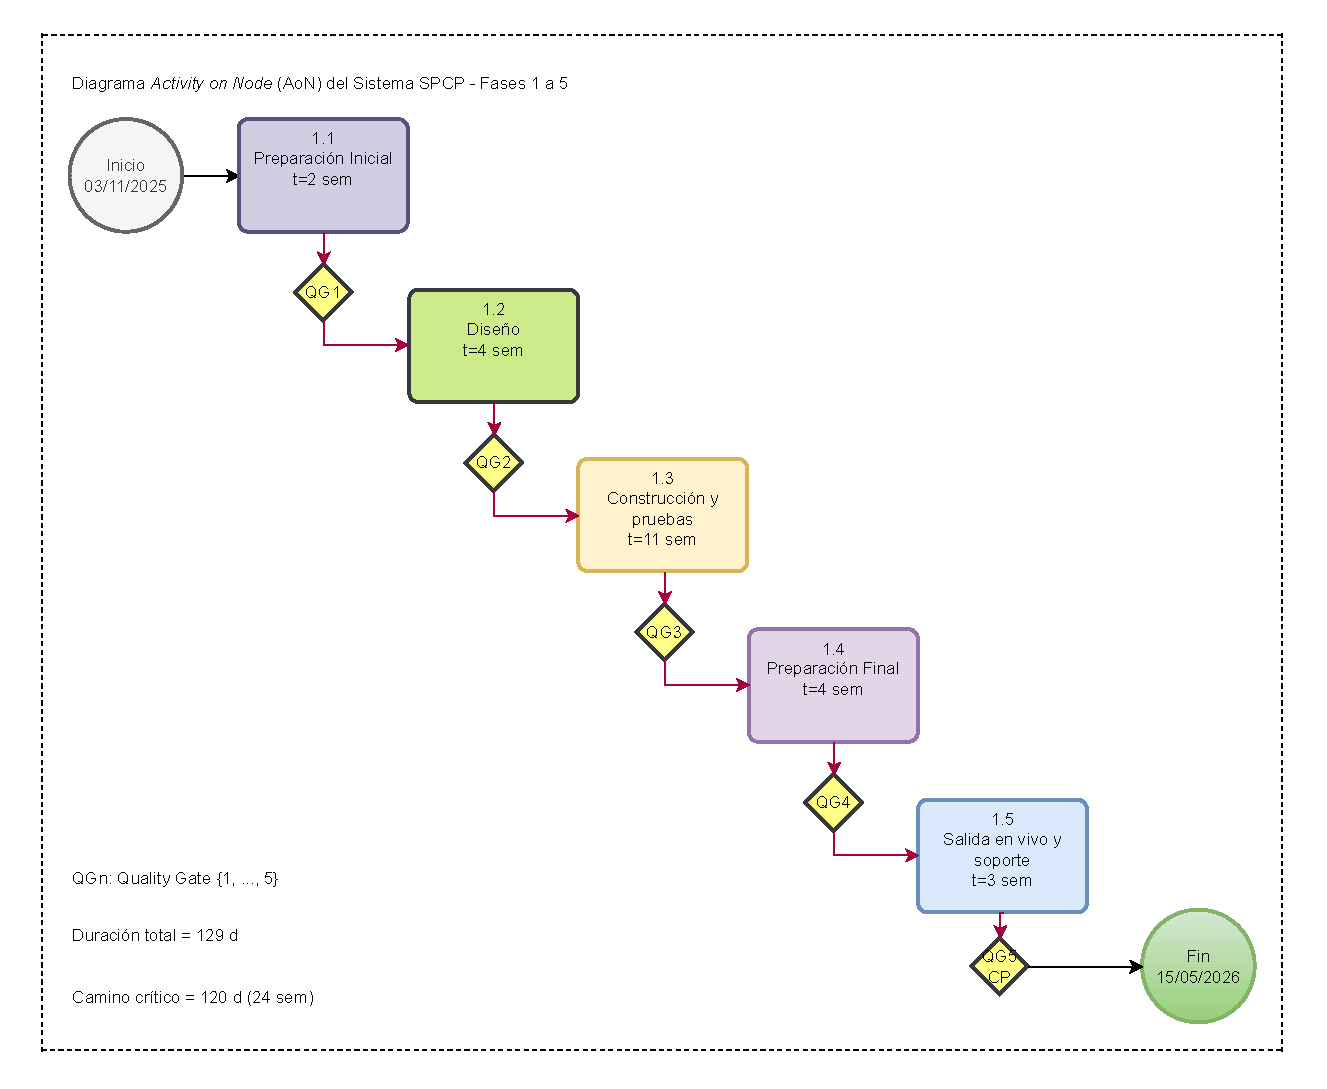
\includegraphics[width=\textwidth]{Figuras/TF_AoN_00.drawio.pdf}
  \caption{Diagrama \textit{Activity on Node} (AoN) del sistema SPCP.}
  \label{fig:TF_AoN_00}
\end{figure}

\FloatBarrier

\begin{figure}[ht]
  \centering
  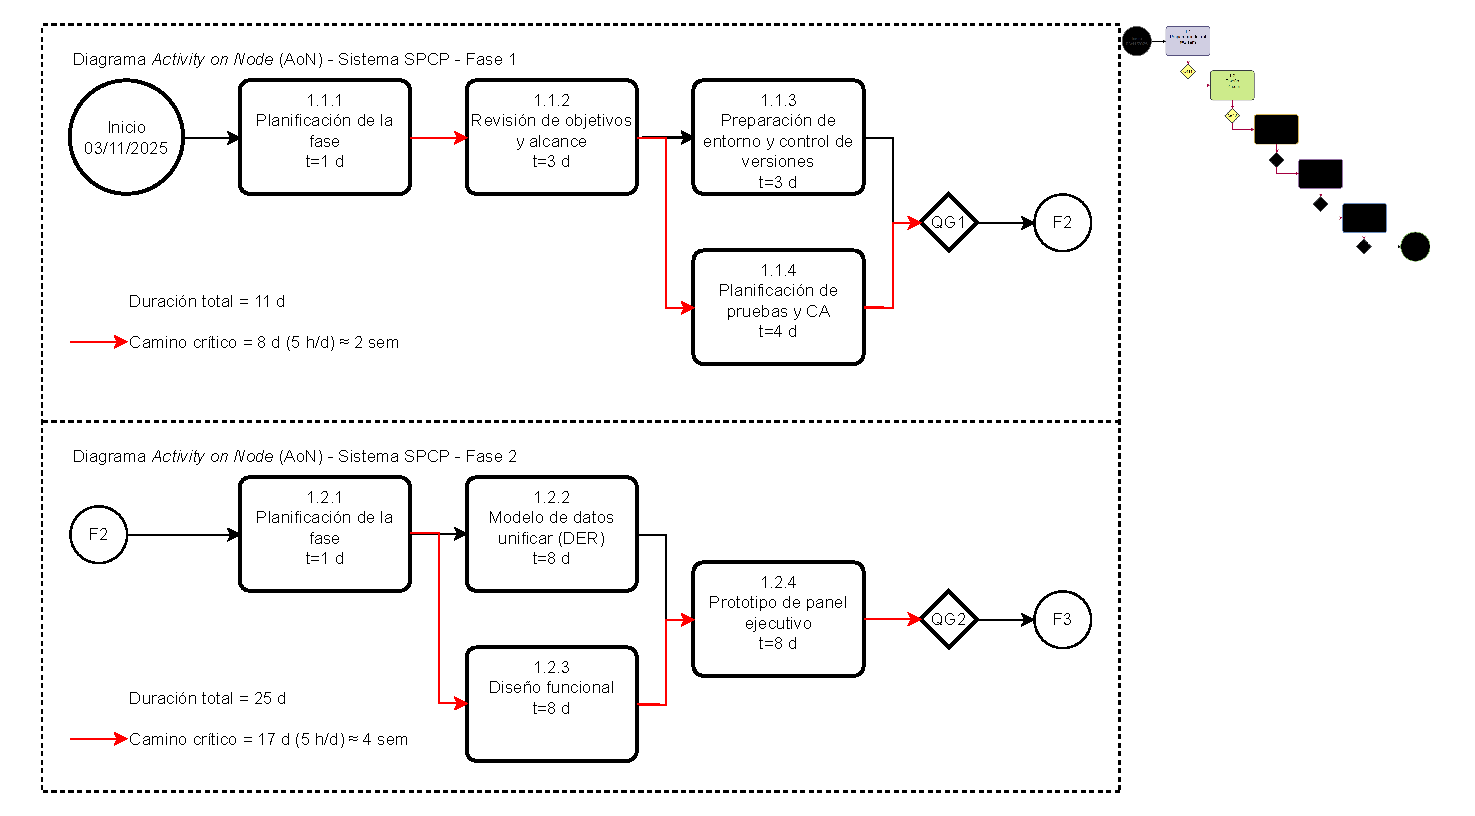
\includegraphics[width=\textwidth]{Figuras/TF_AoN_01_01.drawio.pdf}
  \caption{Diagrama \textit{Activity on Node} (AoN) Fases 1 y 2 del sistema SPCP.}
    \label{fig:TF_AoN_01_01}
\end{figure}

\FloatBarrier

\begin{figure}[ht]
  \centering
  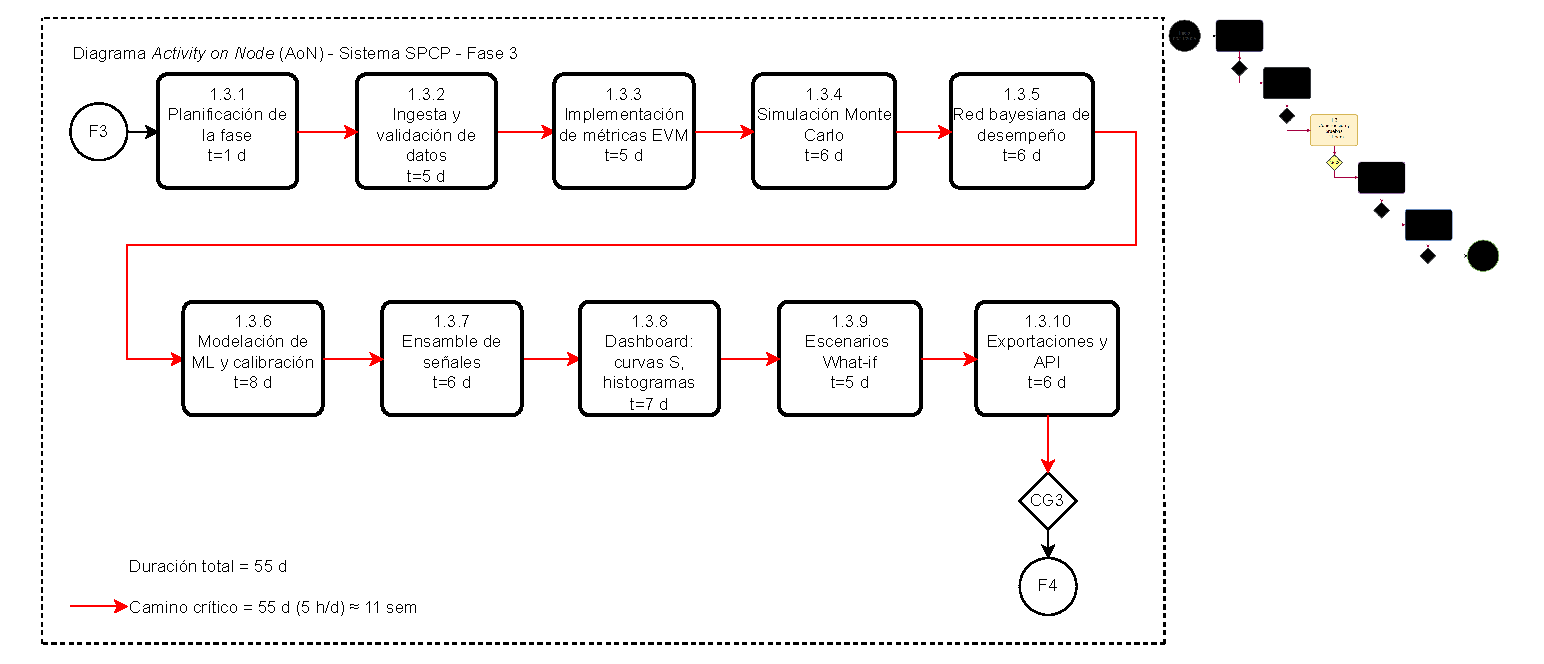
\includegraphics[width=\textwidth]{Figuras/TF_AoN_01_02.drawio.pdf}
    \caption{Diagrama \textit{Activity on Node} (AoN) Fase 3 del sistema SPCP.}
    \label{fig:TF_AoN_01_02}
\end{figure}

\FloatBarrier

\begin{figure}[ht]
  \centering
  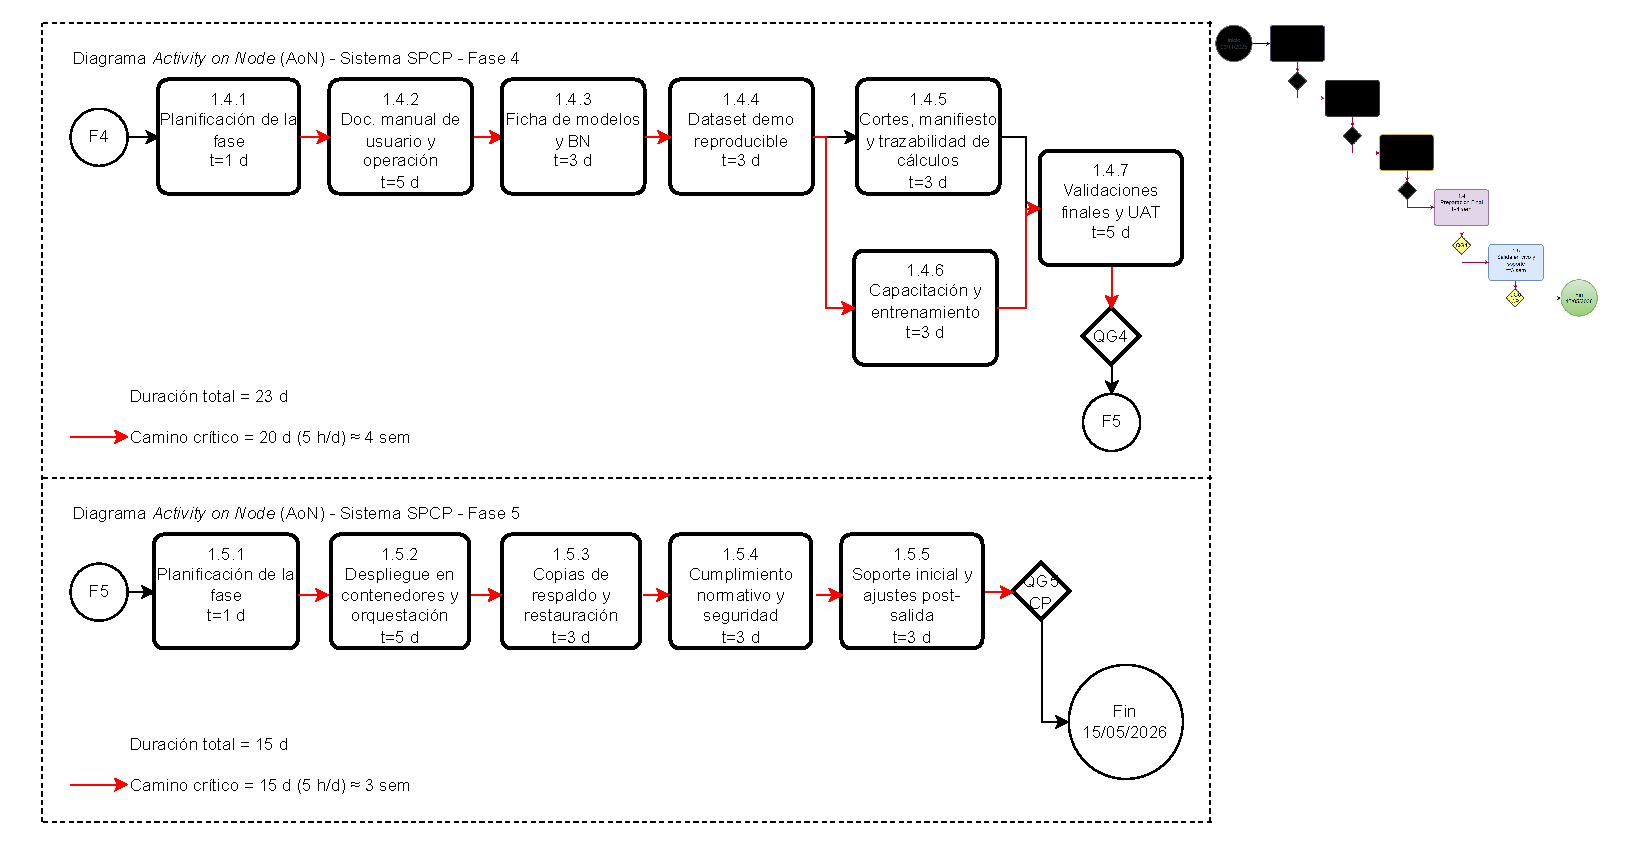
\includegraphics[width=\textwidth]{Figuras/TF_AoN_01_03.drawio.pdf}
  \caption{Diagrama \textit{Activity on Node} (AoN) Fases 4 y 5 del sistema SPCP.}
    \label{fig:TF_AoN_01_03}
\end{figure}

\FloatBarrier

\section{11. Diagrama de Gantt}
\label{sec:gantt}

El diagrama de Gantt constituye la representación temporal detallada del proyecto, derivada de la red AoN previamente definida. 
Mientras que el AoN refleja la lógica de precedencias y el camino crítico entre fases, el Gantt permite asignar duraciones específicas, visualizar la distribución semanal de las actividades y verificar el cumplimiento de hitos. 
En este caso, el cronograma total previsto es de 24 semanas, con fases secuenciales y \textit{quality gates} que actúan como puntos de control obligatorios para avanzar. 
De esta manera, el Gantt se convierte en la herramienta principal de seguimiento y comunicación del avance del SPCP.

\begin{figure}[ht]
  \makebox[\textwidth][c]{%
    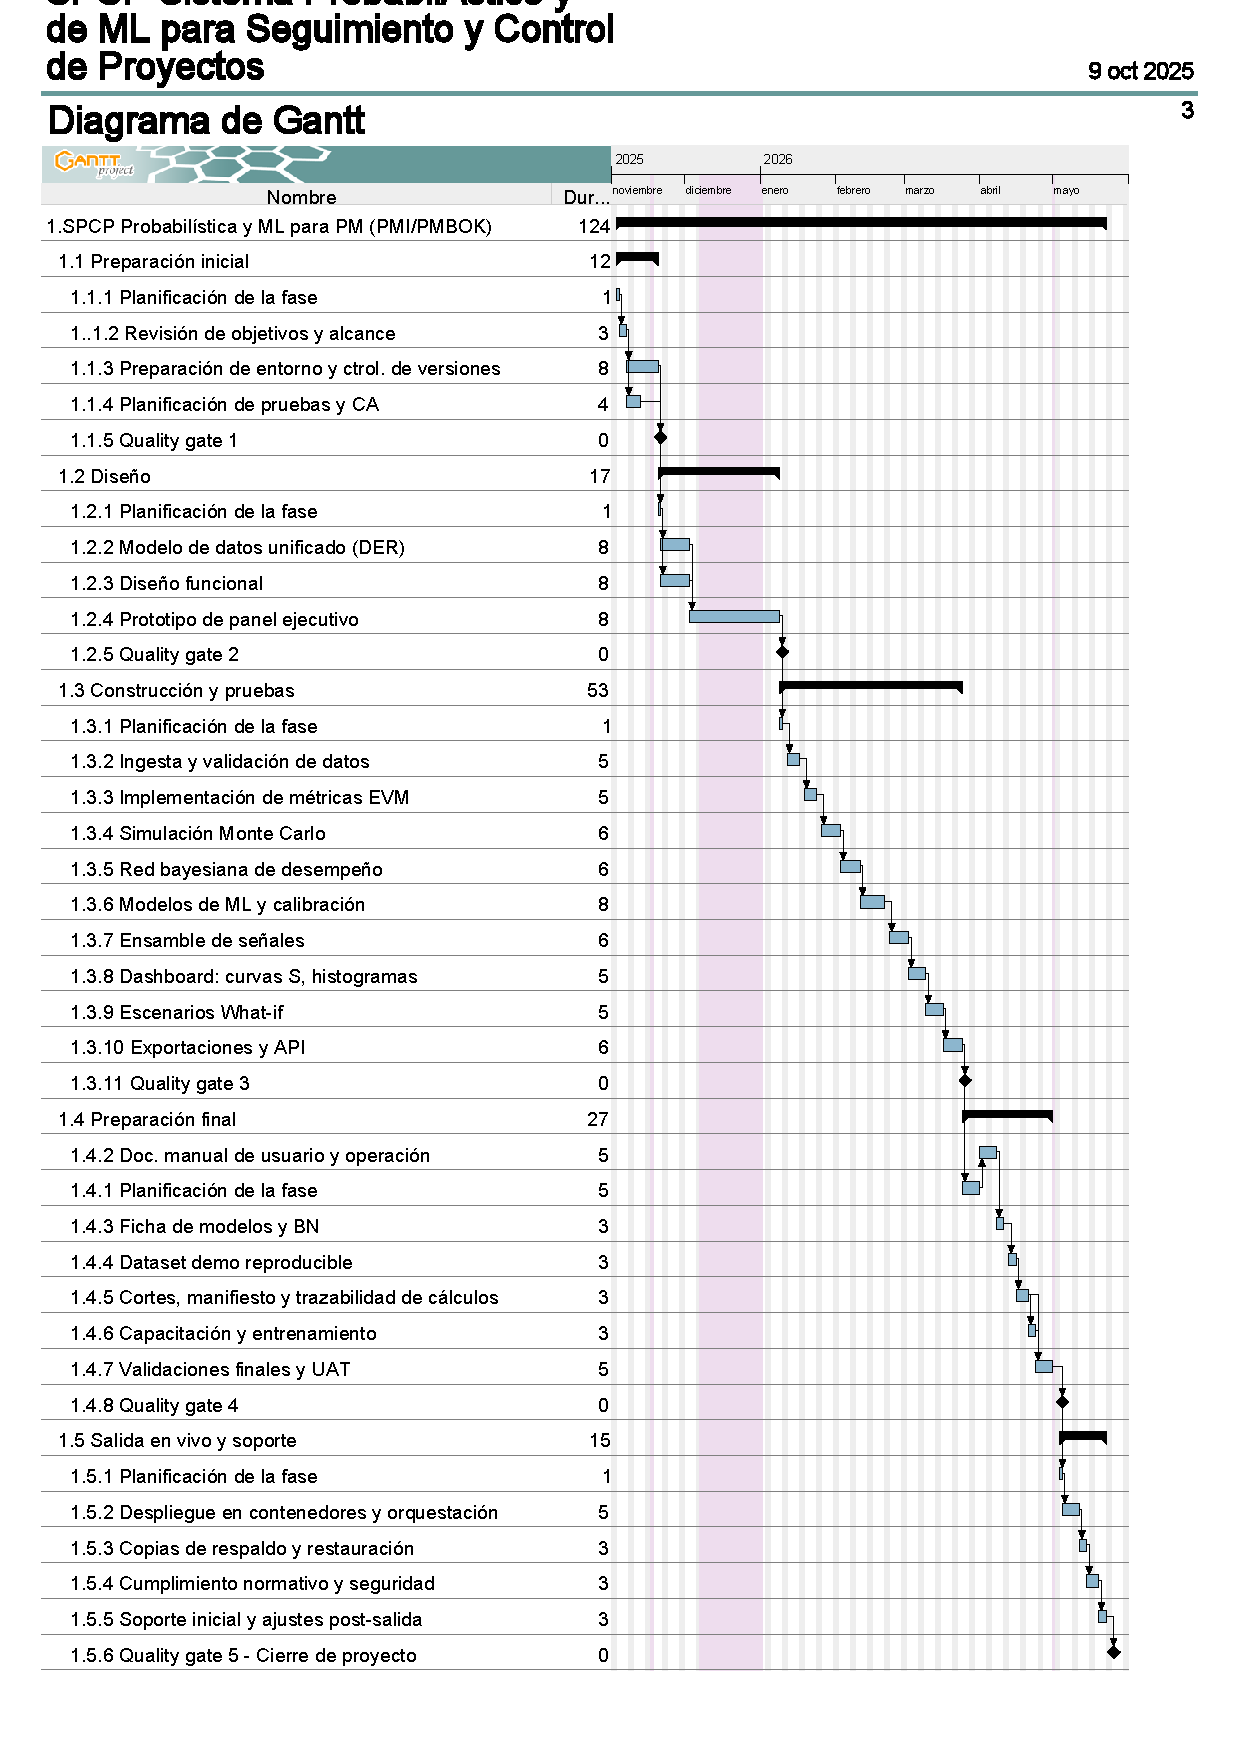
\includegraphics[
      width=1.10\textwidth,  % 25 % más ancho que el texto
      trim=0 30 40 65, clip
    ]{Figuras/CEIA_TF_SPCP_Gantt_p03.pdf}%
  }
  \caption{Cronograma del proyecto representado en diagrama de Gantt.}
  \label{fig:gantt_p03}
\end{figure}
\FloatBarrier

%\begin{figure}[ht]
%  \centering
%  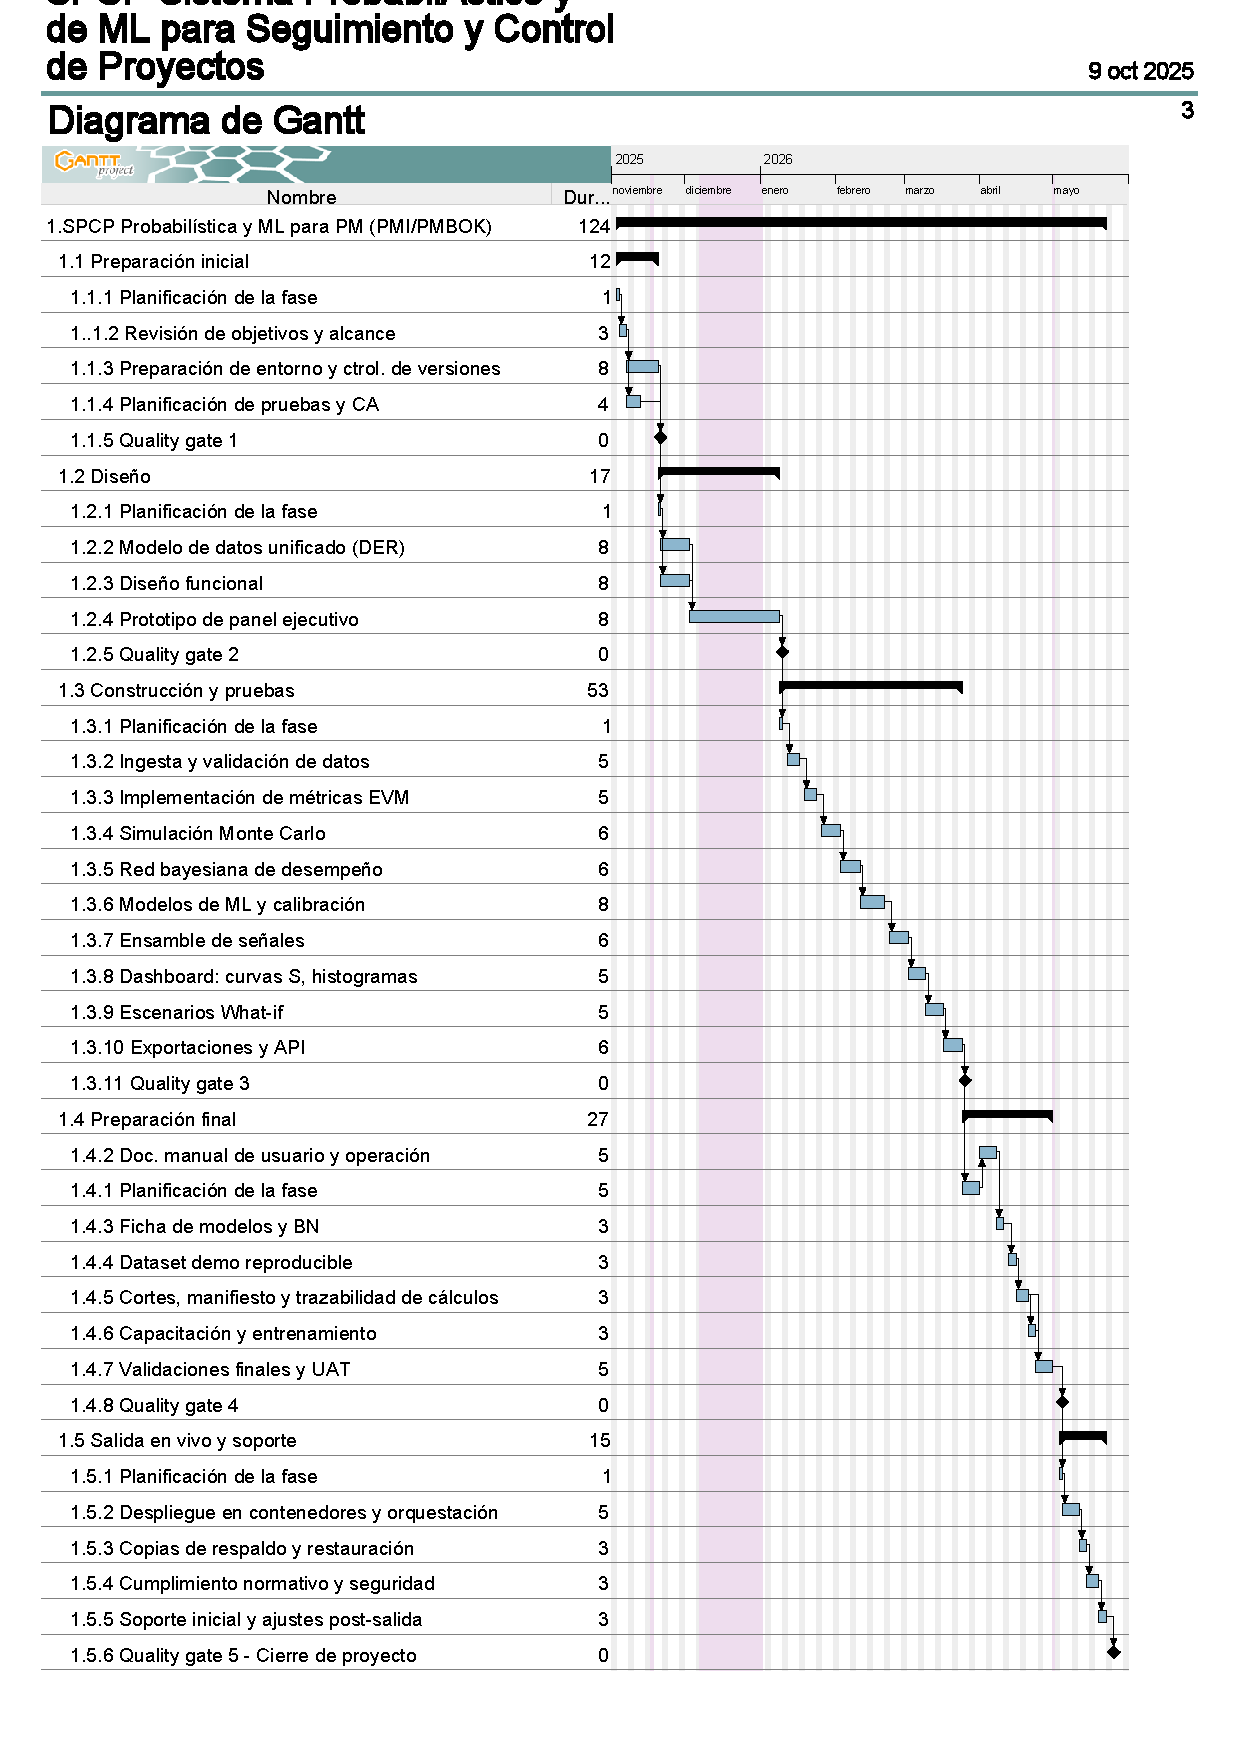
\includegraphics[trim=0 30 15 65,clip,width=\textwidth]{Figuras/CEIA_TF_SPCP_Gantt_p03.pdf}
%  \caption{Cronograma del proyecto representado en diagrama de Gantt.}
%  \label{fig:gantt_p04}
%\end{figure}
%\FloatBarrier


\section{12. Presupuesto detallado del proyecto}
\label{sec:presupuesto}

En la presente sección se detalla el presupuesto del proyecto, discriminado en costos directos e indirectos. 
Los costos directos corresponden al esfuerzo de los perfiles técnicos y de gestión asignados a los paquetes de trabajo definidos en la EDT, expresados en días de dedicación y valor unitario en dólares estadounidenses. Los costos indirectos incluyen aquellos asociados a infraestructura, licencias, soporte administrativo y capacitación, necesarios para garantizar la correcta ejecución del proyecto pero no imputables directamente a un entregable específico. 

De esta forma, se presenta a continuación una tabla resumen con la estructura de desglose de costos, 
indicando cantidades, valores unitarios y subtotales, seguida del total general del proyecto.

\begin{table}[!htbp]
\centering
\scriptsize
\caption{Desglose de costos del proyecto.}
\label{tab:costos}
\begin{tabularx}{\textwidth}{Xccr}
\toprule
\multicolumn{4}{c}{\textbf{COSTOS DIRECTOS}} \\
\midrule
Descripción & Cantidad (días) & Valor unitario [USD] & Valor total [USD] \\
\midrule
Data Scientist & 59 & 200 & 11,800 \\
PM & 31 & 300 & 9,300 \\
QA Tester & 25 & 160 & 4,000 \\
DevOps/MLOps & 23 & 200 & 4,600 \\
Frontend/UI & 21 & 160 & 3,360 \\
Data Engineer & 19 & 160 & 3,040 \\
Compliance & 3 & 160 & 480 \\
\midrule
\textbf{Subtotal directos} & & & \textbf{US\$36,580} \\
\midrule
\multicolumn{4}{c}{\textbf{COSTOS INDIRECTOS}} \\
\midrule
Descripción & Cantidad & Valor unitario [USD] & Valor total [USD] \\
\midrule
Infraestructura y licencias & 1 & 3,000 & 3,000 \\
Soporte administrativo & 1 & 2,000 & 2,000 \\
Capacitaci\'on y entrenamiento & 1 & 1,500 & 1,500 \\
\midrule
\textbf{Subtotal indirectos} & & & \textbf{US\$6,500} \\
\midrule
\textbf{TOTAL PROYECTO} & & & \textbf{US\$43,080} \\
\bottomrule
\end{tabularx}
\end{table}
\FloatBarrier

El valor estimado total del proyecto en moneda local de Argentina (ARS) al 04/10/2025 a TC 1,415.50 ARS/USD es de ARS 60,979,740.00.

\section{13. Gestión de riesgos}
\label{sec:riesgos}

En esta sección se identifican y analizan los principales riesgos asociados al desarrollo e implementación del sistema SPCP.
Cada riesgo fue evaluado en función de su Severidad (S) y probabilidad de Ocurrencia (O) en una escala de 1 a 10,
obteniéndose el Número de Prioridad de Riesgo ($RPN = S \times O$), que permite establecer un orden de criticidad. \\

Se considera un RPN máximo aceptable de 40, por encima del cual se implementarán planes de mitigación específicos para reducir la severidad o probabilidad de ocurrencia.

\begin{table}[ht]
\centering
\scriptsize
\caption{Matriz de riesgos del proyecto (evaluación inicial).}
\label{tab:riesgos}
\begin{tabularx}{\textwidth}{cXccccX}
\toprule
\textbf{ID} & \textbf{Riesgo} & \textbf{S} & \textbf{O} & \textbf{RPN} & \textbf{Prioridad} & \textbf{Acciones de mitigación} \\
\midrule
R1 & Inconsistencia o baja calidad de datos. & 8 & 7 & 56 & 1 &
Definir validaciones automáticas (PK/FK, tipos, acumulados), monitoreo de calidad y alertas tempranas. \\
R3 & Desactualización o pérdida de calibración del modelo. & 8 & 6 & 48 & 2 &
Monitoreo de deriva, umbrales de recalibración y política de reentrenamiento documentada. \\
R2 & Fallas en integración ETL/API. & 7 & 6 & 42 & 3 &
Implementar versionado de esquemas, control de errores y pruebas automáticas en CI/CD. \\
R5 & Retrasos en validación o aprobación de Quality Gates. & 7 & 6 & 42 & 4 &
Planificar QG con anticipación, identificar autorizador alterno y checklist de aceptación previa. \\
R10 & Interpretación errónea de probabilidades y percentiles. & 7 & 6 & 42 & 5 &
Entrenamiento a PMs en lectura de percentiles, leyendas claras en dashboard y ejemplos guiados. \\
R8 & Fallas de versionado o trazabilidad de artefactos. & 8 & 5 & 40 & 6 &
Uso obligatorio de control de versiones (Git), manifiesto + hash en cada corte semanal. \\
R7 & Incumplimiento normativo o exposición de datos sensibles. & 9 & 4 & 36 & 7 &
Cumplimiento ISO 27001 / GDPR, datos anónimos en datasets y auditorías de seguridad. \\
R9 & Baja adopción del sistema por usuarios finales. & 6 & 6 & 36 & 8 &
Pruebas rigurosas, talleres de uso, documentación amigable e incorporación de feedback temprano. \\
R6 & Subestimación del esfuerzo técnico. & 7 & 5 & 35 & 9 &
Incluir margen de seguridad del 25\%, revisión de estimaciones en comité técnico. \\
R4 & Performance insuficiente del sistema (Monte Carlo, paneles). & 6 & 5 & 30 & 10 &
Optimizar código, paralelización, uso de caché y pruebas de carga. \\
\bottomrule
\end{tabularx}
\end{table}
\FloatBarrier

En la siguiente lista se justifican las asignaciones de Severidad (S) y Ocurrencia (O) para los cinco riesgos identificados como críticos (RPN>40):

\begin{itemize}
  \item R1 - Inconsistencia o baja calidad de datos:
  S=8 por su impacto directo en la confiabilidad de los indicadores y simulaciones;
  O=7 por la heterogeneidad y carga manual de las fuentes.
  \item R3 - Desactualización o pérdida de calibración del modelo:
  S=8 por afectar la validez de las predicciones;
  O=6 por la naturaleza cambiante de los datos semanales.
  \item R2 - Fallas en integración ETL/API:
  S=7 porque interrumpe el flujo de datos hacia los modelos;
  O=6 por cambios frecuentes en APIs externas.
  \item R5 - Retrasos en validación o aprobación de Quality Gates:
  S=7 por bloquear el avance entre fases del camino crítico;
  O=6 por la disponibilidad limitada de revisores, aprobadores.
  \item R10 - Interpretación errónea de probabilidades y percentiles:
  S=7 por su impacto en la toma de decisiones;
  O=6 por la complejidad estadística de los resultados.
  \item R8 - Fallas de versionado o trazabilidad:
  S=8 por comprometer la reproducibilidad de los resultados;
  O=5 por posibles errores de configuración o procedimientos manuales.
\end{itemize}

A los valores de S, O y RPN, se los pondera bajo el supuesto de aplicar las acciones de mitigación establecidas, para reflejar el nivel de riesgo residual resultante (S*, O* y RPN*), donde las acciones de mitigación preventivas reducen el impacto (O), mientras que las mitigantes o de contingencia la severidad (S).

En la siguiente tabla se establecen los valores ponderados para los riesgos con RPN>40:

\begin{table}[ht]
\centering
\scriptsize
\caption{Matriz de riesgos del proyecto (S*, O* y RPN*).}
\label{tab:riesgos-RPN-residual}
\begin{tabularx}{\textwidth}{cXccXccc}
\toprule
\textbf{ID} & \textbf{Riesgo} & \textbf{SxO=RPN} & \textbf{Prioridad} & \textbf{Acciones de mitigación} & \textbf{S*} & \textbf{O*} & \textbf{RPN*}  \\
\midrule
R1 & Inconsistencia o baja calidad de datos. & 8x7=56 & 1 &
Definir validaciones automáticas (PK/FK, tipos, acumulados), monitoreo de calidad y alertas tempranas. & 5 & 6 & 30 \\
R3 & Desactualización o pérdida de calibración del modelo. & 8x6=48 & 2 &
Monitoreo de deriva, umbrales de recalibración y política de reentrenamiento documentada. & 6 & 6 & 36 \\
R2 & Fallas en integración ETL/API. & 7x6=42 & 3 & 
Implementar versionado de esquemas, control de errores y pruebas automáticas en CI/CD. & 4 & 6 & 24 \\
R5 & Retrasos en validación o aprobación de Quality Gates. & 7x6=42 & 4 &
Planificar QG con anticipación, identificar autorizador alterno y checklist de aceptación previa. & 5 & 5 & 25 \\
R10 & Interpretación errónea de probabilidades y percentiles. & 7x6=42 & 5 &
Entrenamiento a PMs en lectura de percentiles, leyendas claras en dashboard y ejemplos guiados. & 5 & 6 & 30 \\
\bottomrule
\end{tabularx}
\end{table}
%\FloatBarrier

Se representa la matriz de riesgos en un \textit{heatmap}, donde se visualizan las combinaciones de Severidad y Ocurrencia, y se destaca en rojo los que requieren atención prioritaria.

\begin{figure}[H]
  \centering
  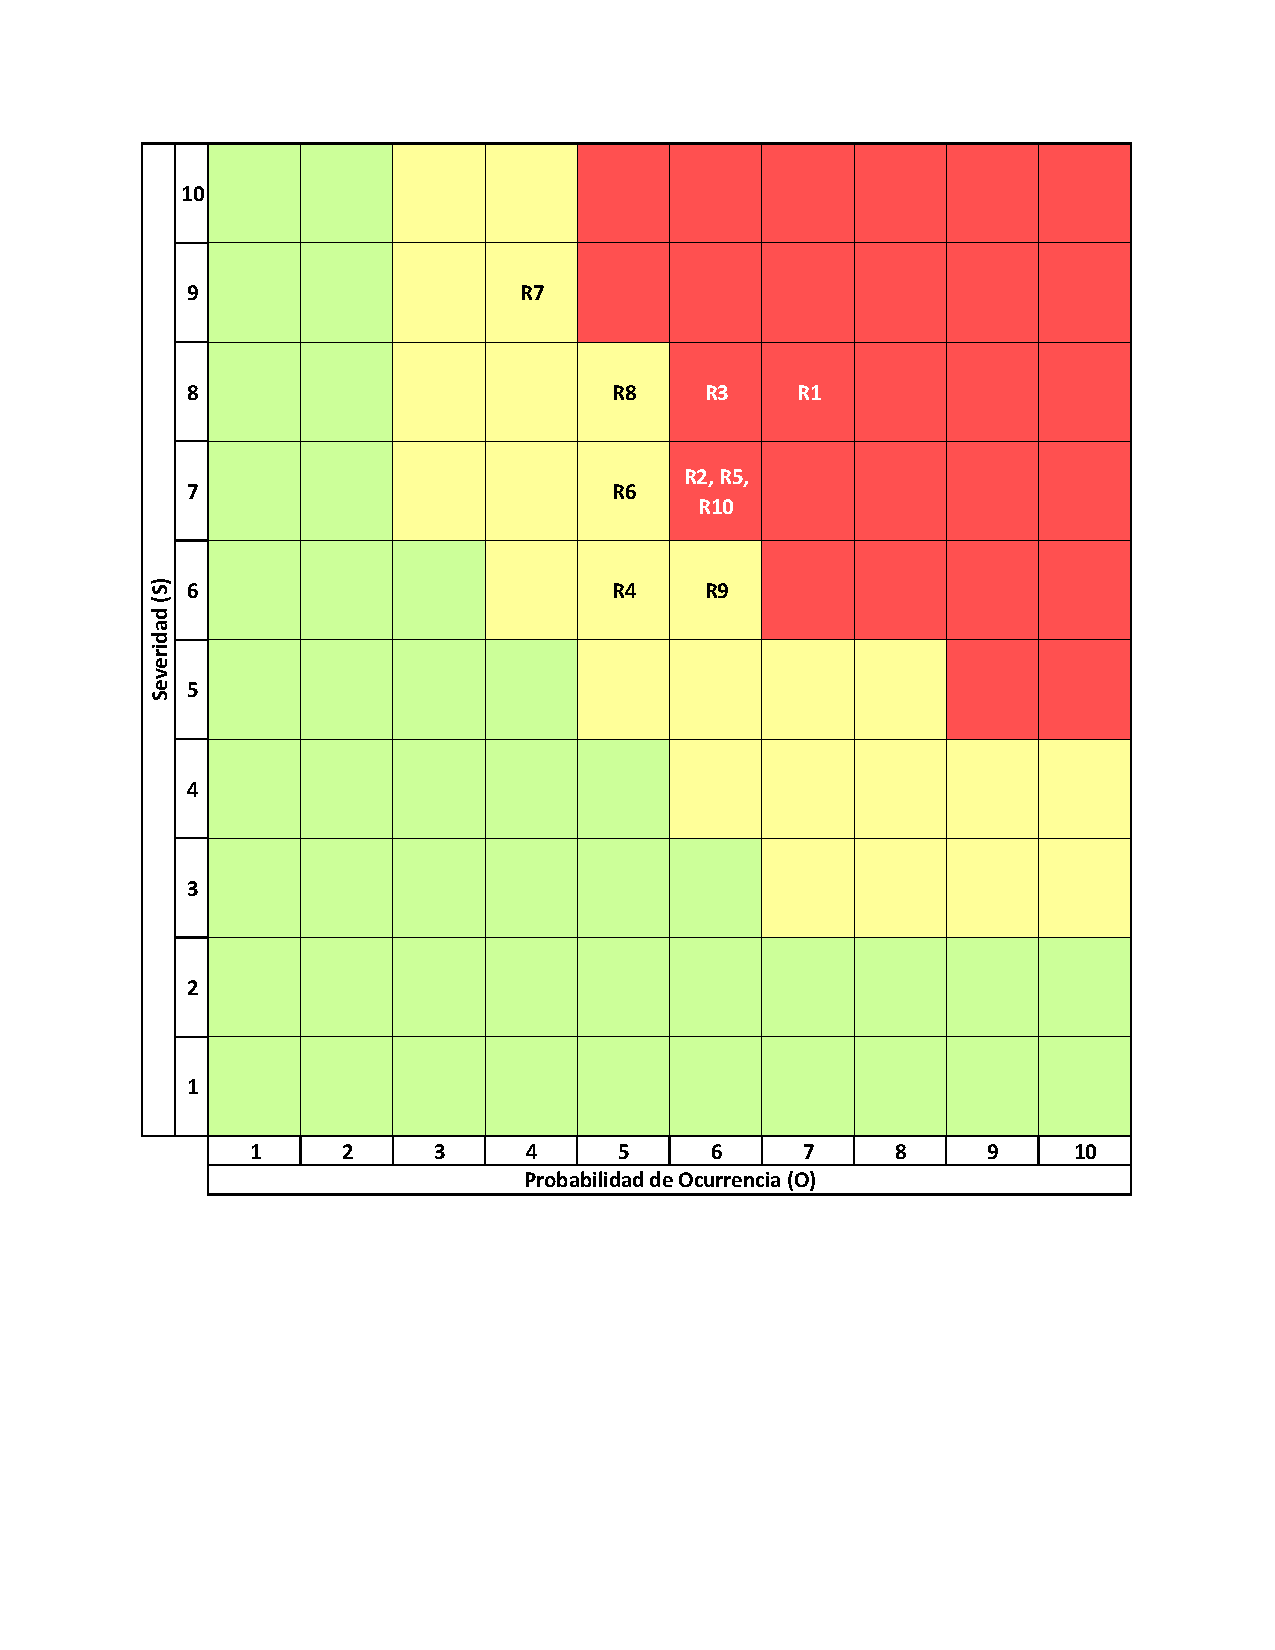
\includegraphics[trim=65 213 65 65,clip,width=0.65\textwidth]{Figuras/TF_Heatmap_Risk.pdf}
  \caption{Mapa de calor de riesgos según el valor del RPN (rojo indica críticos >40).}
  \label{fig:TF_Heatmap_Risk}
\end{figure}
\FloatBarrier

\section{14. Gestión de la calidad}
\label{sec:calidad}

La gestión de la calidad del proyecto SPCP tiene como propósito asegurar que los entregables cumplan con los requerimientos funcionales, técnicos y normativos definidos, manteniendo trazabilidad, verificabilidad y aceptación formal por parte del cliente.  

Para cada requerimiento seleccionado se definen acciones de verificación y validación.  
Las acciones de verificación consideran al entregable como una "caja blanca", es decir, se examina su funcionamiento interno mediante revisión de código, simulaciones, cálculos, análisis de resultados, pruebas unitarias o revisión de hojas de datos.  
Las acciones de validación, en cambio, tratan al entregable como una "caja negra", evaluando su comportamiento externo, la percepción del usuario, la conformidad del cliente o la coherencia con los objetivos del proyecto.  
En ambos casos se contemplan consultas con expertos, mediciones, o contrastes con datos reales o simulados según corresponda.

A continuación, se describen la verificación y validación correspondientes a 13 requerimientos seleccionados.

\begin{itemize}

\item Req \#FR-03 - Cálculo EVM (CPI, SPI, CV, SV, EAC, TCPI).
  \begin{itemize}
    \item Verificación: revisión de fórmulas en el código y pruebas con dataset controlado (valores conocidos); comparación contra resultados calculados manualmente y contra una planilla de referencia; pruebas unitarias de cada indicador y de casos borde.
    \item Validación: contraste con series históricas provistas por el cliente; revisión con el comité técnico de la coherencia de tendencias (CPI/SPI) y aceptación de resultados en un caso real de negocio.
  \end{itemize}

\item Req \#FR-04 - Monte Carlo (cronograma) con PERT (a,m,b) y $\geq 10{,}000$ corridas; reporte de P50/P80/P90 y $P(\text{Finish}>\text{Baseline})$.
  \begin{itemize}
    \item Verificación: ejecución con semilla fija para reproducibilidad; chequeo de estabilidad de percentiles ante repeticiones; validación de la transformación PERT y de la propagación de duraciones; pruebas de tolerancias sobre P50/P80/P90 con escenarios sintéticos.
    \item Validación: demostración al cliente de escenarios de cronograma y coherencia de percentiles con expectativas; aceptación formal del comportamiento probabilístico en una WBS de prueba.
  \end{itemize}

\item Req \#FR-05 - Red bayesiana (desempeño) para estimar $P(\text{EAC}>\text{BAC})$ con observables (CPI, SPI, exposición de riesgo, cambios, retrabajo, demoras proveedor).
  \begin{itemize}
    \item Verificación: revisión de estructura y supuestos de la red; pruebas de posterior predictivo y sensibilidad de nodos; chequeos con datos simulados controlando direcciones de efecto.
    \item Validación: revisión guiada con el cliente (PM) sobre los resultados inferidos y su interpretación; acuerdo de que los cambios en observables se reflejan en \textit{posteriors} de manera esperable.
  \end{itemize}

\item Req \#FR-07 - Fusión de señales (EVM + Bayes + ML) mediante ensamble para EAC final y probabilidad de sobrecosto.
  \begin{itemize}
    \item Verificación: comparación de salidas individuales vs. ensamble; revisión de pesos o metamodelo (\textit{stacking}) y chequeo de mejora en error y estabilidad; pruebas de consistencia cuando falta alguna señal.
    \item Validación: presentación de desempeño consolidado al comité; aceptación de que el ensamble no degrada y aporta robustez frente a métodos individuales.
  \end{itemize}

\item Req \#FR-08 - Visualización ejecutiva (KPIs, curvas S, histograma y tabla ejecutiva exportable).
  \begin{itemize}
    \item Verificación: verificación de presentación y actualización de los datos con datasets de distintos tamaños; comparación de los valores mostrados respecto al backend y pruebas de exportación CSV/PDF/PNG.
    \item Validación: sesión con usuarios clave para evaluar legibilidad, navegabilidad y comprensión de KPIs; ajustes menores y aceptación en UAT.
  \end{itemize}

\item Req \#TEST-02 - Contrato de datos en CI: el build debe fallar ante cambios incompatibles.
  \begin{itemize}
    \item Verificación: integración de validación de esquema (tipos, PK/FK, requeridos) en el pipeline; inyección de cambios incompatibles simulados y comprobación de fallo controlado.
    \item Validación: demostración al cliente del proceso de rechazo con evidencia de logs y política de versionado de esquema aprobada.
  \end{itemize}

\item Req \#TEST-05 - Validación de modelos de ML (\textit{k-fold}, MAE/RMSE, curva de calibración).
  \begin{itemize}
    \item Verificación: ejecución del pipeline con particiones fijas; revisión de métricas por \textit{fold} y promedio; verificación de calibración y tests de no fuga temporal.
    \item Validación: presentación de métricas consolidadas y gráficos de calibración al cliente; aceptación de umbrales acordados.
  \end{itemize}

\item Req \#UI-05 - Explicabilidad combinada.
  \begin{itemize}
    \item Verificación: chequeo de consistencia de valores SHAP con perturbaciones controladas; validación de sensibilidad en nodos de la red bayesiana; prueba de sincronía entre texto y visual.
    \item Validación: revisión con usuarios avanzados de si las explicaciones permiten entender drivers; aprobación de ejemplos guiados.
  \end{itemize}

\item Req \#DEV-05 - MLOps.
  \begin{itemize}
    \item Verificación: pruebas de registro y versionado (modelo, \textit{features}, semillas); restauración desde un \textit{snapshot}; ejecución de reentrenamiento según umbrales.
    \item Validación: simulación de ciclo de vida completo ante el cliente con trazabilidad de artefactos; aceptación del procedimiento.
  \end{itemize}

\item Req \#DATA-01 - Modelo unificado (DER vigente).
  \begin{itemize}
    \item Verificación: validación automática del esquema contra el diccionario; rechazo de columnas extra y reporte de discrepancias; pruebas con datasets deliberadamente inválidos.
    \item Validación: verificación conjunta con el cliente de la correspondencia DER-dataset en un corte real; conformidad de estructura y dominios.
  \end{itemize}

\item Req \#REG-01 - Cumplimiento de privacidad de datos.
  \begin{itemize}
    \item Verificación: revisión del módulo de anonimización y de los mecanismos de cifrado de credenciales; auditoría interna de logs para confirmar la ausencia de datos sensibles en outputs.
    \item Validación: validación con el responsable de cumplimiento y el cliente de que los datos utilizados y exportados cumplen las políticas de privacidad vigentes; aceptación formal mediante checklist de cumplimiento.
  \end{itemize}

\item Req \#DOC-03 - Manual de usuario.
  \begin{itemize}
    \item Verificación: revisión editorial y técnica del documento para asegurar coherencia entre pantallas, pasos y funcionalidades; pruebas cruzadas por un integrante ajeno al desarrollo.
    \item Validación: sesión de revisión guiada con usuarios reales siguiendo los procedimientos del manual; incorporación de observaciones y aprobación final del cliente.
  \end{itemize}

\item Req \#TEST-10 - Pruebas de aceptación de usuario (UAT).
  \begin{itemize}
    \item Verificación: ejecución de los escenarios definidos en el plan de pruebas con registro de resultados y evidencias.
    \item Validación: sesión de pruebas con usuarios finales y cliente; firma del acta de aceptación tras confirmar cumplimiento de todos los casos de prueba.
  \end{itemize}

\end{itemize}


\section{15. Procesos de cierre}    
\label{sec:cierre}

El proceso de cierre del proyecto SPCP tiene como objetivo consolidar los resultados alcanzados, verificar el cumplimiento del plan aprobado, documentar las lecciones aprendidas y reconocer el esfuerzo del equipo y de los interesados.  
Las siguientes pautas establecen las actividades que se llevarán a cabo en la reunión final de evaluación y cierre en el \textit{Quality Gate} 5 - Cierre del proyecto.

\subsection{Revisión del cumplimiento del Plan de Proyecto}
La revisión del cumplimiento del plan estará a cargo del responsable del proyecto (PM), con la participación del \textit{Data Scientist} líder y del responsable técnico.  
El procedimiento consistirá en:
\begin{itemize}
  \item Comparar las fechas reales de cada hito y entregable contra las planificadas en el cronograma base (\textit{Gantt}).
  \item Contrastar los indicadores EVM finales (CPI, SPI, EAC) con los valores objetivo definidos al inicio.
  \item Revisar los entregables aprobados y verificar la cobertura de los requerimientos funcionales, no funcionales y normativos.
  \item Registrar las desviaciones detectadas y clasificarlas según su causa (alcance, cronograma, recursos o calidad).
\end{itemize}

El resultado de esta revisión quedará documentado en un acta de cumplimiento firmada por el PM y validada por el comité académico del proyecto.

\subsection{Lecciones aprendidas, técnicas y problemas identificados}
El análisis de las técnicas y procedimientos empleados será coordinado por el PM con la colaboración de los responsables técnicos de cada área (ETL, ML, MLOps, UI, QA).  
El procedimiento incluirá:
\begin{itemize}
  \item Identificar las metodologías y herramientas que resultaron más útiles (por ejemplo, CI/CD, validaciones automáticas, control de versiones, simulaciones Monte Carlo).
  \item Documentar aquellas prácticas o enfoques que resultaron poco eficientes o redundantes, junto con las razones identificadas.
  \item Describir los principales problemas surgidos durante el desarrollo (integración de datos, calibración de modelos, coordinación de \textit{Quality Gates}) y las soluciones aplicadas.
  \item Consolidar la información en un documento de “Lecciones aprendidas” para referencia en futuros proyectos.
\end{itemize}

El acta de lecciones aprendidas será publicada en el repositorio del proyecto y formará parte del material de referencia del SPCP.

\subsection{Agradecimientos y reconocimiento al equipo}
La organización del acto de agradecimiento estará a cargo del PM, con apoyo administrativo y logístico del área de operaciones académicas.  
Durante este evento se presentarán los resultados finales, se reconocerá el aporte de los integrantes del equipo de trabajo y se agradecerá a los colaboradores externos y asesores académicos.  
Los gastos asociados (logística, materiales, refrigerios) serán financiados con cargo al presupuesto del proyecto en el rubro de indirectos $"$Gastos administrativos$"$ asignado al Trabajo Final.

Finalmente, se elaborará un informe de cierre que consolidará toda la documentación del proyecto (actas, entregables finales, métricas de desempeño, resultados de pruebas, lecciones aprendidas y reconocimientos), constituyendo la versión definitiva del SPCP para archivo y referencia.

\end{document}